\documentclass[10pt]{beamer}
\usepackage{amsmath,amsfonts}	% use math symbols
\usepackage{helvet}
\usepackage{graphicx} % insert images
\usepackage{url} % insert urls
\usepackage{textpos} % package for the positioning
\usepackage{caption}
\usepackage{subcaption}
\usepackage{mathtools}
\usetheme{Pittsburgh} % change theme
\usecolortheme{dove}
%% NEW COMMANDS
\def\ci{\perp\!\!\!\perp}
\def\dep{\perp\!\!\!\perp\!\!\!\!\!\!\!/\,\,\,\,}
\begin{document}

%% MAKE TITLE
\title{Indicative Support Vector Clustering}
\subtitle{Application on Anomaly Detection}
\author{Huang Xiao} %\\ \small{xiaohu@in.tum.de} }%\thanks{Funded by ARAMiS project}}
%\and Author2 \inst{1} }
%\and Author3 \inst{2}}
\institute[Technische Universit\"at M\"unchen]
{ 
	%\inst{1} 
	Chair of IT Security (I20) \\Department of Informatics \\Technische Universit\"at M\"unchen 
	%\and
	%\inst{2} Cloud Service Lab\\Fraunhofer AISEC
}

\date{\today}
\maketitle

%% CHANGE THE DEFAULT TEMPLATE
% position the logo
\addtobeamertemplate{frametitle}{}{%
\begin{textblock*}{100mm}(-0.3cm,-0.4cm)
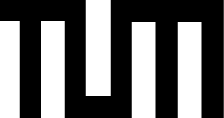
\includegraphics[height=0.53cm,width=0.9cm,keepaspectratio]{imgs/tumlogo_bw}
\end{textblock*}}

\AtBeginSection[] {
	\frame<beamer>{ 
		\frametitle{Overview}   
		\tableofcontents[currentsection] 
 	}
 }
 % add frame number
%\setbeamertemplate{footline}{%
  %\raisebox{5pt}{\makebox[\paperwidth]{\hfill\makebox[10pt]{\scriptsize\insertframenumber}}}}

%% START PRESENTATION
\section{Recap on fast KDE}
\subsection{What have I done before?}
\begin{frame}{Fast KDE}
\begin{block}{To find the outliers...}
Data points are scattered in "some" space, e.g., Euclidean space, Hilbert space.
Outliers are those points with lower density, which can be measured by Kernel Density Estimation (\textit{KDE}).
\end{block}
\begin{columns}
\hskip10pt
\begin{column}{.35\textwidth}
\begin{figure}
\centering
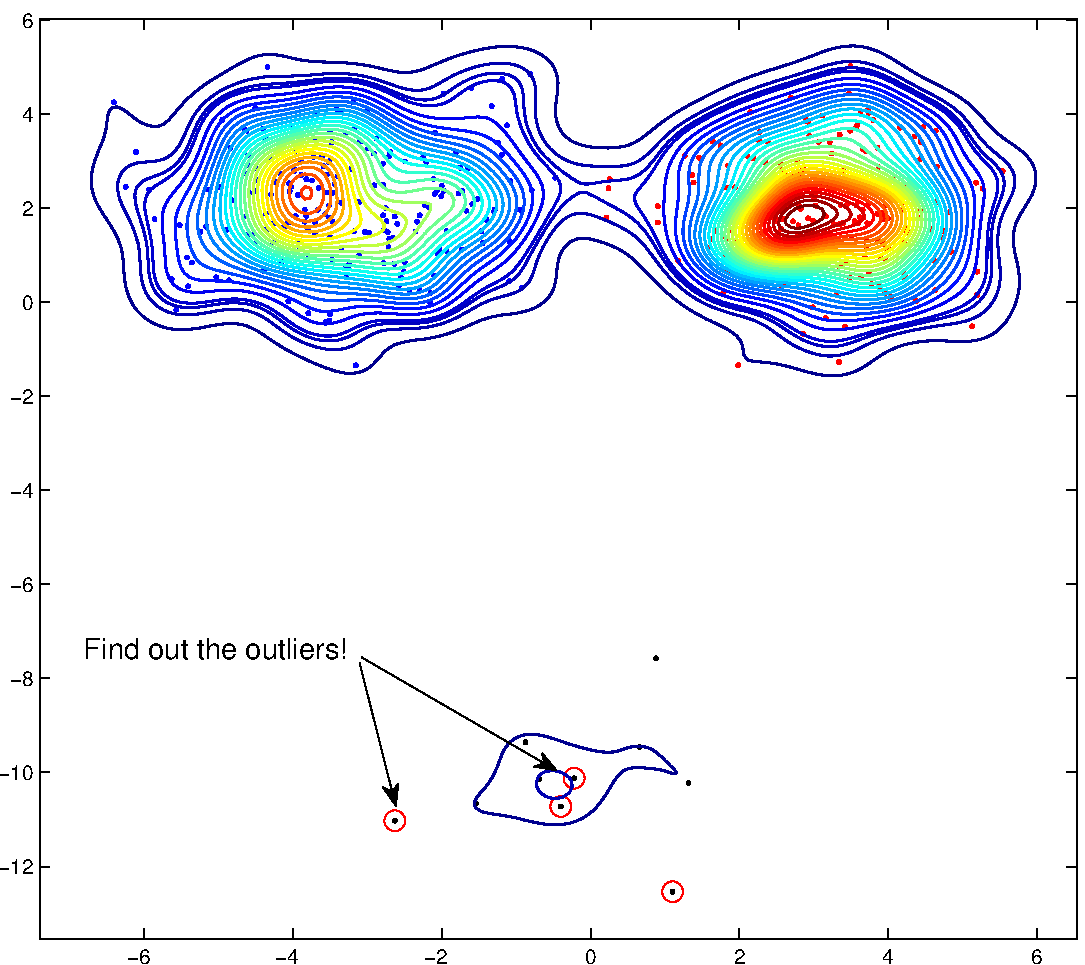
\includegraphics[scale=0.25]{imgs/outliers_density}
\end{figure}
\end{column}
\begin{column}{.65\textwidth}
\begin{center}
\small
The kernel density estimate of $x^*$ is
\[
f(x^*) = \frac{1}{nh}\sum^n_{i=1}K(\frac{x^* - x_i}{h})
\]
\color{red} Testing density is too much overhead!
\end{center}	
\end{column}
\end{columns}
\end{frame}


\begin{frame}{Fast KDE: use clustering}
\begin{flushleft}
Clustering the data points first
\end{flushleft}
\begin{columns}
\hskip10pt
\begin{column}{.35\textwidth}
\begin{figure}
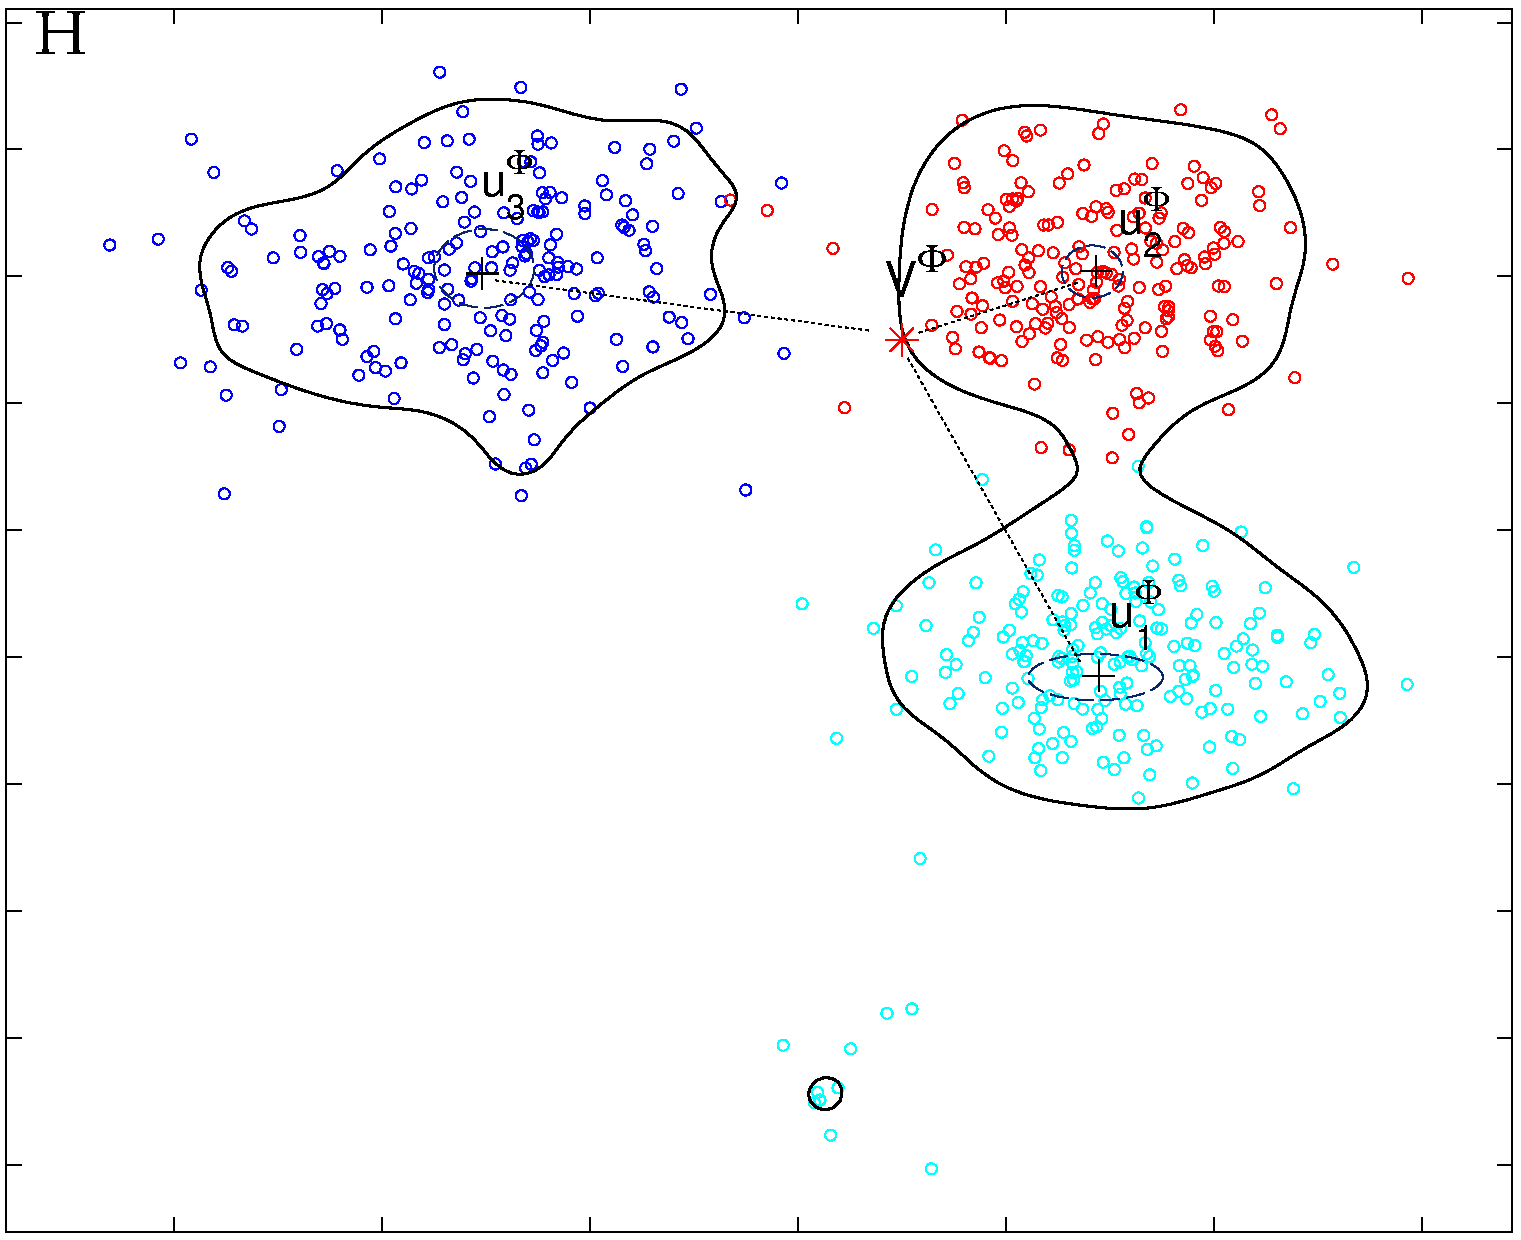
\includegraphics[width=3.5cm, height=3.5cm]{imgs/kclust}
\end{figure}
\end{column}
\begin{column}{.65\textwidth}
\small
\centering
Averaging on $m$ cluster centers:
\[
\hat{V}^\Phi=\frac{1}{m}\sum_{i=1}^m w_i\Phi_i(x_s)
\]
which is more efficient.\\ \vskip20pt \pause
\alert{BUT, lose too much precision, when $m$ is small}
\end{column}
\end{columns}
\end{frame}


\subsection{Compromised too much?}
\begin{frame}{Problems}
\begin{itemize}
\item Density approximation only rely on cluster centers.
\item Require to define how many clusters we have, i.e., $m=?$
\item Outliers are averaged equally, not robust.
\item We also need to integrate user feedback.
\end{itemize}
\end{frame}

\begin{frame}{Another clustering?}
\begin{block}{Solution}
Instead of looking for the cluster center, we look for the cluster bounds using support vectors. 
\end{block}
\end{frame}
%\begin{frame}{Causal Inference Overview}
%\begin{figure}
%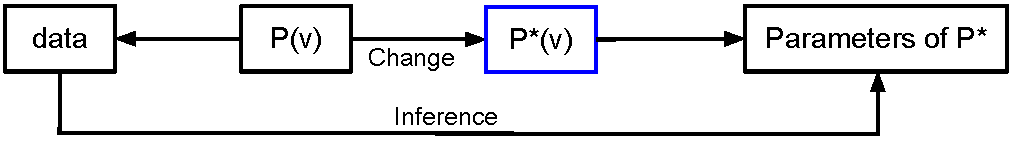
\includegraphics[scale=0.6]{imgs/causalInf}
%\end{figure}
%\begin{itemize}
%\item What if $P$ has shifted itself to $P^*$?
%\item<2-> \textbf{Key factors:} Causes, Changes, and Invariants . 
%\item<2-> Inference of $P^*$ and reasoning of changes. 
%\end{itemize}
%\end{frame}
%\begin{frame}{What makes Causal Inference interesting?}
%\begin{itemize}
%\item Human understands the world in terms of causes and effects.
%\item Empirical science is about establishing causes.
%\item Causal inference gives a mathematical language for causal
%statements, and tools to solve causal problems formally.
%\item Alternative exercising to decision making, reasoning, etc.
%\end{itemize}
%%\begin{alertblock}{Note}
%%Causal Inference has fundamental difference with machine learning
%%\end{alertblock}
%\end{frame}
%\subsection{Causal Graphical Model}
%\begin{frame}{Association}
%\begin{itemize}
%\item Now we want to find out what \alert{causes} lung cancer
%\end{itemize} \pause
%\begin{columns}
%\begin{column}{0.5\textwidth}
%\begin{table}
%\centering
%\begin{tabular}{|c|c|c|c|}
%\hline
%& & \multicolumn{2}{|c|}{Lung cancer}\\\hline
%smoking & yellow teeth & yes & no\\\hline
%yes & yes & 100 & 400\\\hline
%yes & no & 100 & 400\\\hline
%no & yes & 1 & 450\\\hline
%no & no & 9 & 8540\\\hline
%\end{tabular}
%\caption{Data observations from 10000 people}
%\end{table}
%\end{column}\hfill
%\begin{column}{0.5\textwidth}
%\vspace*{-0.5in}
%\begin{figure}
%\centering
%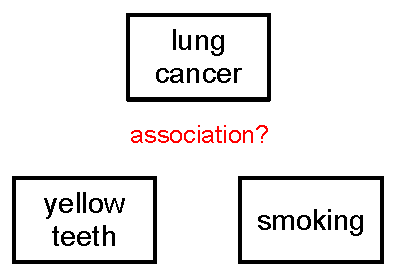
\includegraphics[scale=0.6]{imgs/smokepl}
%\end{figure}
%\end{column}
%\end{columns}
%\end{frame}
%\begin{frame}{Measurements of Association}
%\textbf{To find out associations among variables}
%\begin{itemize}
%\item Mutual information (Information theory)
%\item Pearson (linear) correlation
%\item Spearman's rho (rank correlation)
%\item Effect size between two variables
%\item Many others
%\end{itemize}
%\end{frame}
%\begin{frame}{Observations from Data}
%\textbf{Obviously}
%\begin{itemize}
%\item \textit{yellow teeth} and \textit{lung cancer} are associated.
%\end{itemize}\pause
%\alert{\textbf{But...}}
%\begin{itemize}
%\item Bleaching the teeth does not help reduce the probability
%of getting lung cancer.
%\end{itemize}\pause
%\begin{alertblock}{Caution!}
%Correlation does not imply Causation
%\end{alertblock}
%\end{frame}
%\begin{frame}{Statistical Implication}
%\begin{block}{Reichenbach's \textit{Common Cause Principle}}
%If $X$ and $Y$ are correlated, then either $X$ causes $Y$ or $Y$ causes $X$ or they share a latent common cause $Z$.
%\end{block}
%\begin{figure}
%\setcounter{subfigure}{0}
%	\centering
%	\begin{subfigure}[H]{0.3\textwidth}
%		\centering
%		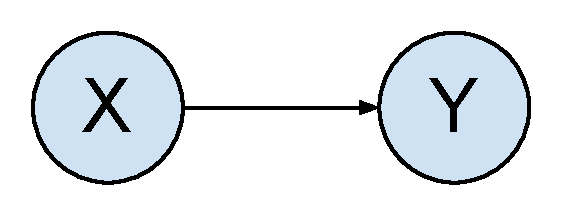
\includegraphics[scale=0.3]{imgs/x2y}
%		\caption{$X$ causes $Y$}
%		%\label{}	
%	\end{subfigure}
%	\begin{subfigure}[H]{0.3\textwidth}
%		\centering
%		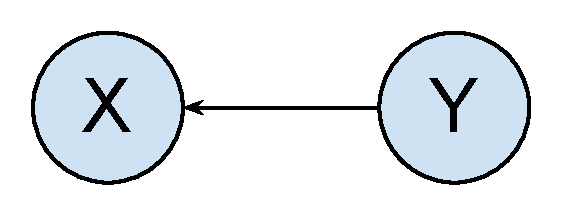
\includegraphics[scale=0.3]{imgs/y2x}
%		\caption{$Y$ causes $X$}
%		%\label{}	
%	\end{subfigure}
%	\begin{subfigure}[H]{0.3\textwidth}
%		\centering
%		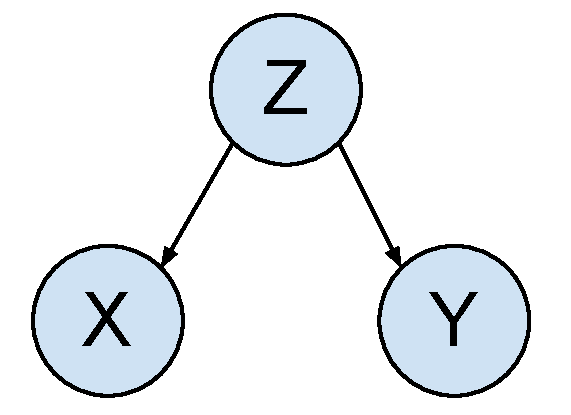
\includegraphics[scale=0.3]{imgs/z2xy}
%		\caption{A common latent cause $Z$}
%		%\label{}	
%	\end{subfigure}
%\end{figure}\pause
%\begin{itemize}
%\item<+-|alert@+> It links causality with probability
%\end{itemize}
%\end{frame}
%\begin{frame}{Functional Causal Model (pearl et al.)} 
%\begin{itemize}[<+->]
%\item A set of variables (factors) $\left\lbrace X_1,\ldots,X_n \right\rbrace$
%\item Directed acyclic graph $\mathcal{G}$ with vertices $\left\lbrace X_1,\ldots,X_n \right\rbrace$
%\item Parents of node $X_i$ in $\mathcal{G}$ are its direct causes
%\item $X_i=f_i(Parents(X_i),\epsilon_i)$, where $\left\lbrace\epsilon_1,\ldots,\epsilon_n\right\rbrace$ are jointly independent noises
%\item The above entails a joint probability distribution $P(X_1,\ldots,X_n)$
%\item Problems are twofold:
%      \begin{enumerate}
%		\item How is the $P$ like?
%		\item Can we recover $\mathcal{G} from P$? 
%	\end{enumerate}
%\item[] \begin{textblock*}{200mm}(0.6\textwidth,-2cm)
%		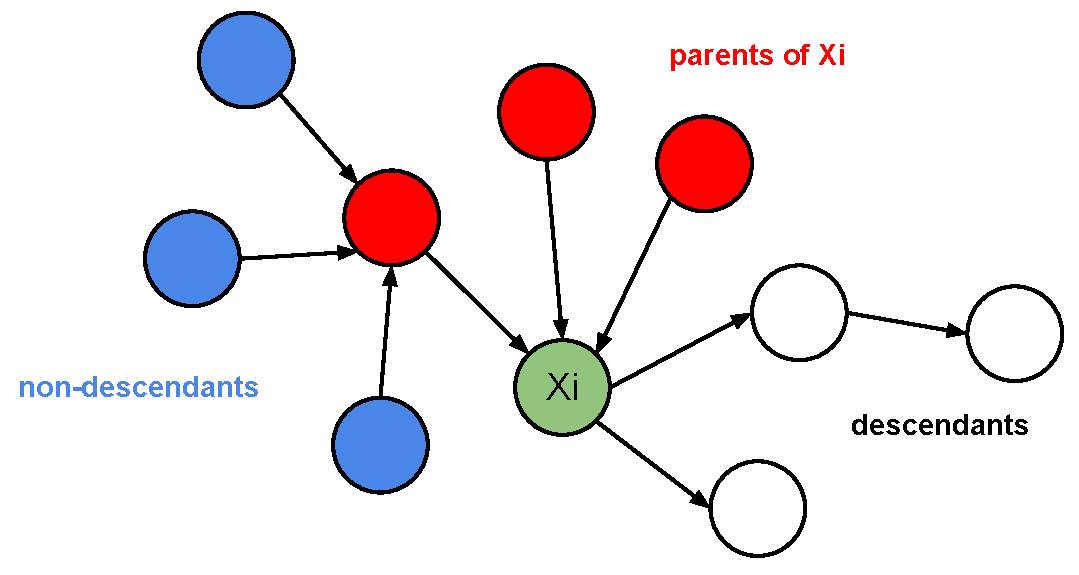
\includegraphics[scale=0.25]{imgs/causalgm}
%	\end{textblock*}
%\end{itemize}
%\end{frame}
%\begin{frame}{Functional Causal Model, ctd.}
%The following are equivalent:
%\begin{itemize}
%\item A functional causal model exists
%\item Local causal Markov condition: $X_i$ is statistically independent of its non-descendants given $X_i$'s parents
%\item Global Causal Markov condition: \textbf{d-separation} characterize the set of independences over all the observables
%\item Factorization: $P(X_1,\ldots,X_n)=\prod_iP(X_i\,|\,Parents(X_i))$
%\end{itemize}
%\end{frame}
%\begin{frame}{Learning causation from Data?}
%\begin{block}{Question}
%Given observational data, can we infer $\mathcal{G}$?
%\end{block}
%\begin{itemize}
%\item \textbf{Simple answer:} impossible without additional information
%\item Possible with interventions (outside force, empirical treatment, etc.)
%\item By conditional independence tests, \textit{Markov equivalence class} containing $\mathcal{G}$ can be learned. \alert{But}, it fails in simplest 2-nodes case.
%\item 2-nodes case can be tackled applying residual dependence test. (see Hoyer et al.)
%\end{itemize}
%\end{frame}
%\begin{frame}{Markov Equivalence Class}
%\textbf{Simplest case with three variables}
%\begin{itemize}
%\item[]<1-> \begin{figure}
%\setcounter{subfigure}{0}
%			\begin{subfigure}[H]{0.4\textwidth}
%			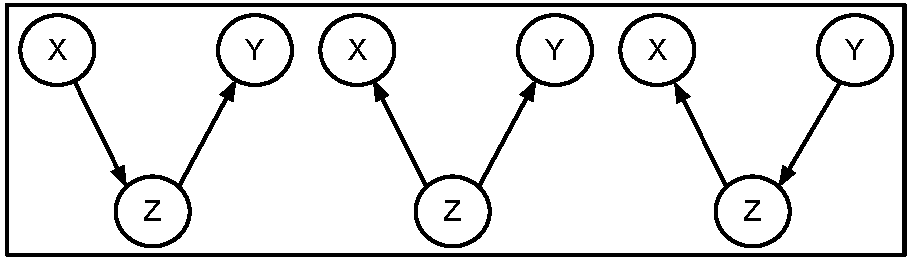
\includegraphics[scale=0.4]{imgs/eqv}
%			\caption{Equivalence}
%			\end{subfigure}\hfill
%			\begin{subfigure}[H]{0.3\textwidth}
%			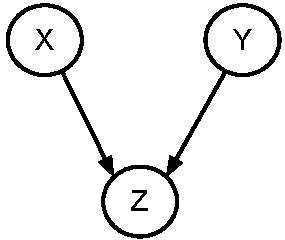
\includegraphics[scale=0.4]{imgs/noneqv}
%			\caption{Non-equivalence}
%			\end{subfigure}
%		\end{figure}
%\item<2-> Samples can be explained by all graphs in equivalence class
%\item<3-> For example:
%\begin{table}
%\centering
%\begin{tabular}{|c|c|}
%\hline
%Equivalence class & Non-equivalence class \\\hline
%$Dep(X,Z\,|\,\emptyset)$ & $Dep(X,Z\,|\,\emptyset)$\\\hline
%$Dep(Y,Z\,|\,\emptyset)$ & $Dep(Y,Z\,|\,\emptyset)$\\\hline
%$Dep(X,Y\,|\,\emptyset)$ & \alert{$Ind(X,Y\,|\,\emptyset)$}\\\hline
%$Ind(X,Y\,|\,Z)$ & \alert{$Dep(X,Y\,|\,Z)$}\\\hline
%\end{tabular}
%\end{table}	
%\end{itemize}
%\end{frame}
\section{Support Vector Clustering}
\subsection{How it works in kernel space?}
\begin{frame}{How it works}
\begin{block}{In a mysterious space...}
Data points can be structured into a hypersphere where low density points are fading away.
\end{block}
\vskip20pt
\begin{figure}
\centering
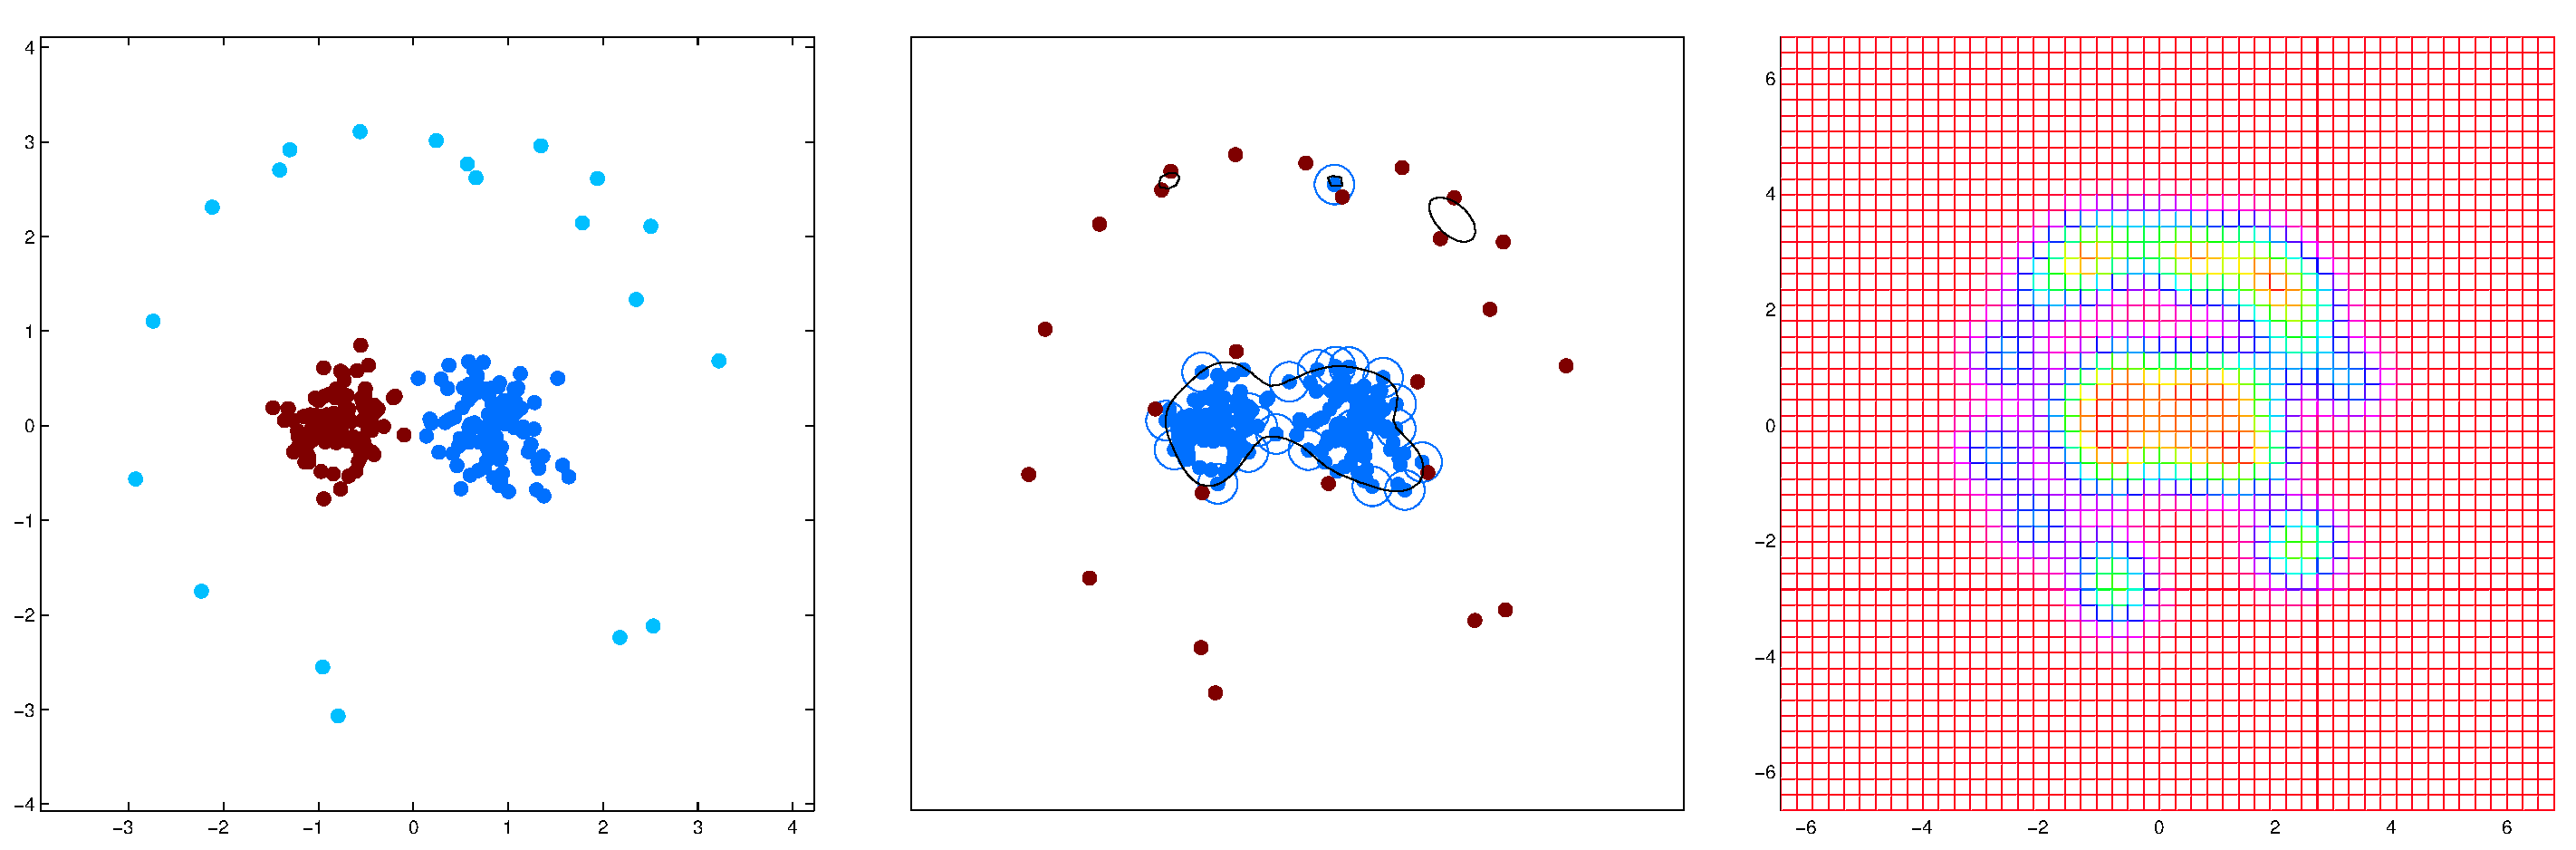
\includegraphics[scale=0.22]{imgs/svn_sample}
\caption{Support vector clustering example}
\end{figure}
\end{frame}

\begin{frame}{Cutting the low density area}
\begin{columns}
\begin{column}{.5\textwidth}
Support Vector Machine
\begin{figure}
\hskip-30pt
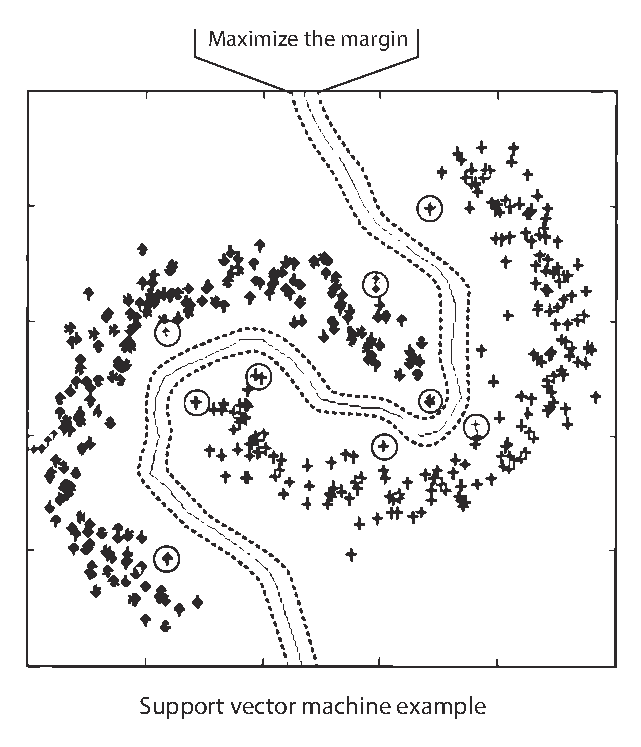
\includegraphics[scale=0.35]{imgs/svm_sample.pdf}
\end{figure}
\color{blue}Maximize the margin!
\end{column}
\begin{column}{.5\textwidth}
Support Vector Clustering
\begin{figure}
\hskip-30pt
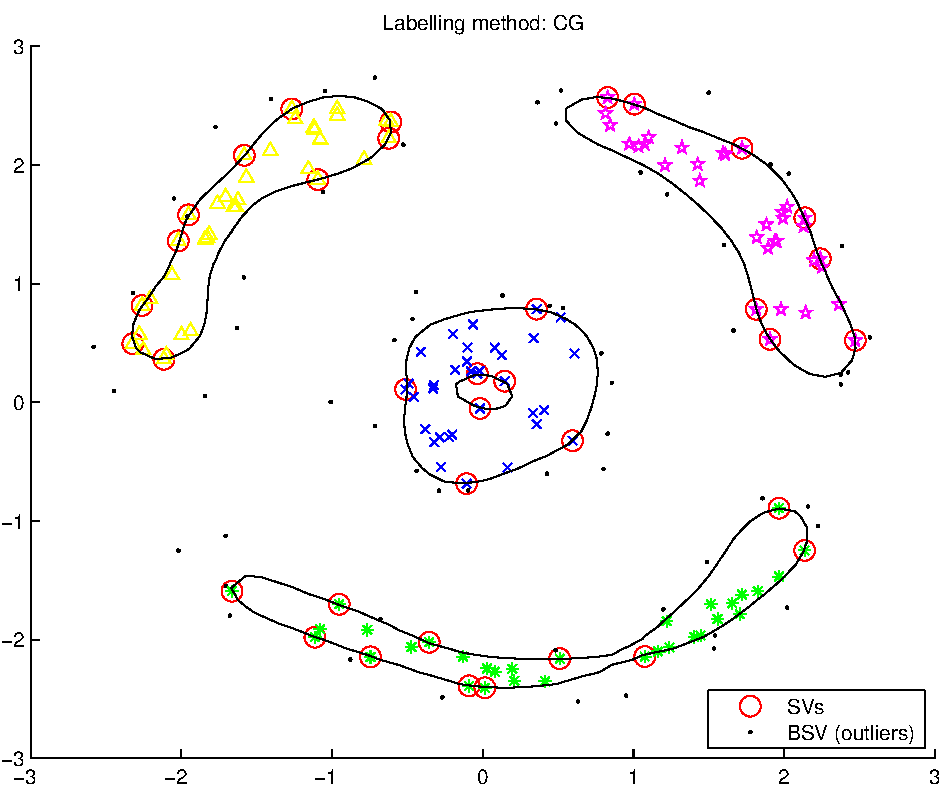
\includegraphics[scale=0.2]{imgs/svc1.pdf}\\ \hskip-30pt
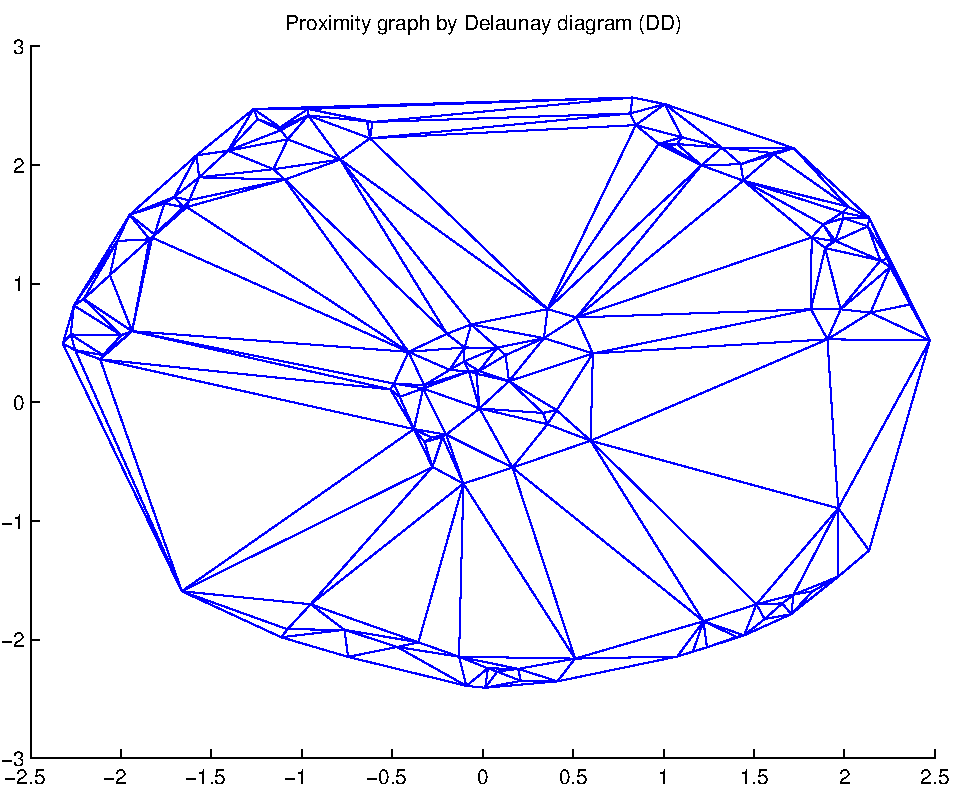
\includegraphics[scale=0.2]{imgs/svc1st.pdf}
\end{figure}
\color{blue}Minimize the hypersphere
\end{column}
\end{columns}
\end{frame}

\subsection{SVC Theory}
\begin{frame}{Optimization problem}
Looking for a smallest sphere $\left\langle R, g\right\rangle$ enclosing all data points:
\begin{align}
\label{eq:svc1}
&\min \left(R^2 + C\sum \xi_i\right)	\nonumber \\
\text{subject to}\quad &  \| \Phi(x_j) - g\|^2 \leq R^2 + \xi_j,\; \forall j \nonumber \\
& \xi_j \geq 0 \nonumber
\end{align} 
\begin{description}
\item[$R$]: the radius of the hypersphere
\item[$g$]: the center of the hypersphere
\item[$\| \Phi(x_j) - g\|^2$]: the distance of point $x_j$ to center $g$
\item[$\xi_i$]: slackness variables
\item[$C$]: punishments on slackness
\end{description}
\pause
\vskip20pt
\color{red} Minimizing the ball allowing part of points fade way (slackness).
\end{frame}

\begin{frame}{Properties}
\begin{columns}
\begin{column}{0.65\textwidth}
\begin{itemize}
\item The minimal ball with $R$ is cutting the data points from low density area.
\item Normal data points are inside the ball.
\item Support vectors $X_{SVs}$ are directly on the sphere.
\item Outliers with $\xi_i > 0$ is outside the ball.
\item The clustering bound is a natural threshold finding out the outliers. 
\item No need to define the $m$ (\#clusters)
\end{itemize}
\end{column}
\begin{column}{.35\textwidth}
\begin{figure}
\hskip-20pt
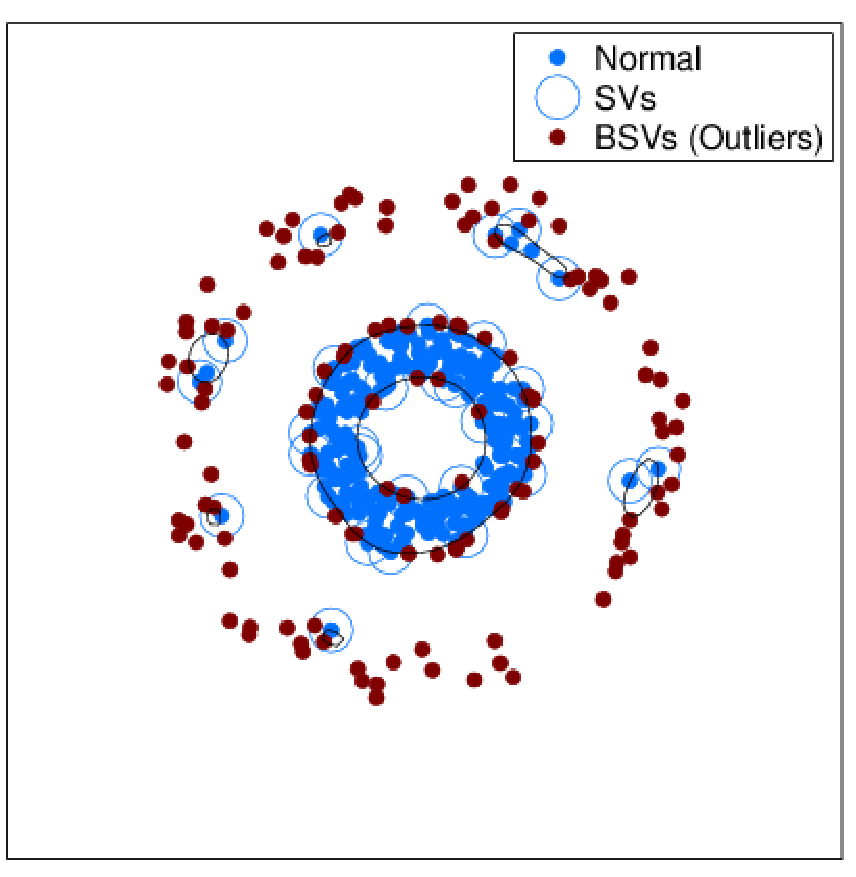
\includegraphics[scale=0.3]{imgs/svc3.pdf}
\end{figure}
\end{column}
\end{columns}
\end{frame}


\subsection{Connection to KDE}
\begin{frame}{From the cluster bound to centers}
\begin{figure}
\centering
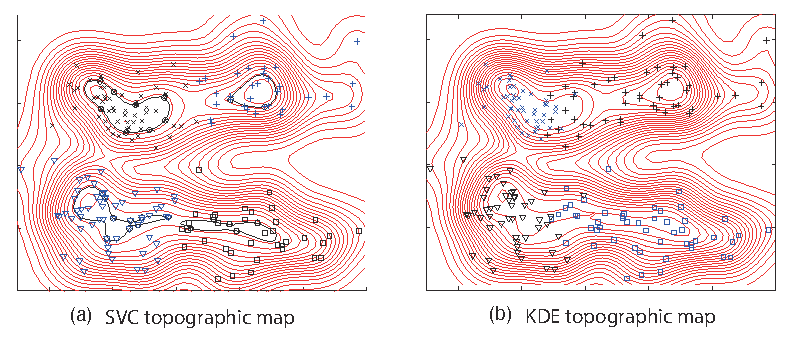
\includegraphics[scale=0.7]{imgs/svc_kde.pdf}
\end{figure}
\begin{itemize}
\item Shrink the cluster bounds to centers.
\item Allow all the points to be repelled outside the ball.
\end{itemize}
\end{frame}
\begin{frame}{Advantages over KDE}
\begin{itemize}
\item Computational easier
\item Define a core region rather than a peak
\item Topographically more reliable
\item Global optimal solution rather than many local maxima  
\end{itemize}
\end{frame}

\subsection{Open problems}
\begin{frame}{Optimization results}
Finally we got...
\vskip10pt
\[
g=\sum\beta_{\mathrm{sv}}\Phi(x_{\mathrm{sv}}) + \sum\beta_{\mathrm{bsv}}\Phi(x_{\mathrm{bsv}}) + \sum\beta_{\mathrm{in}}\Phi(x_{\mathrm{in}}),
\]
\begin{center}
$0 < \beta_{\mathrm{sv}} < C$, $\beta_{\mathrm{bsv}}=C$, $\beta_{\mathrm{in}}=0$
\end{center}
\pause
\vskip40pt
\color{red} Note: the ball center $g$ is still heavily biased by outliers ($\beta_{\mathrm{bsv}}$)
\end{frame}
\begin{frame}{Problems}
\begin{itemize}
\item Only deal with low density outliers
\item Learning is not robust ($g$ is biased)
\item We need to integrate user feedbacks
\end{itemize}
\end{frame}
%\begin{frame}{Statistical Implication}
%\begin{block}{Reichenbach's \textit{Common Cause Principle}}
%If $X$ and $Y$ are correlated, then either $X$ causes $Y$ or $Y$ causes $X$ or they share a latent common cause $Z$.
%\end{block}
%\begin{figure}
%\setcounter{subfigure}{0}
%	\centering
%	\begin{subfigure}[H]{0.3\textwidth}
%		\centering
%		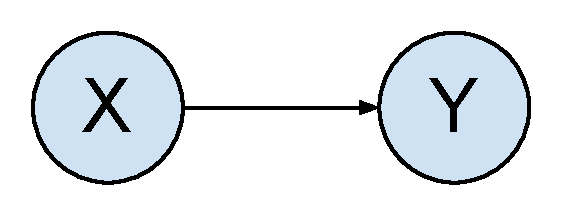
\includegraphics[scale=0.3]{imgs/x2y}
%		\caption{$X$ causes $Y$}
%		%\label{}	
%	\end{subfigure}
%	\begin{subfigure}[H]{0.3\textwidth}
%		\centering
%		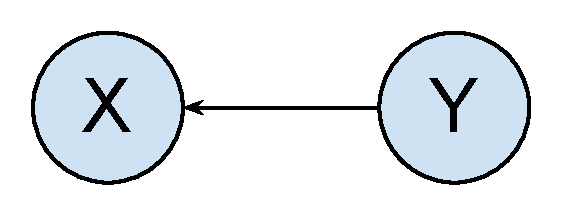
\includegraphics[scale=0.3]{imgs/y2x}
%		\caption{$Y$ causes $X$}
%		%\label{}	
%	\end{subfigure}
%	\begin{subfigure}[H]{0.3\textwidth}
%		\centering
%		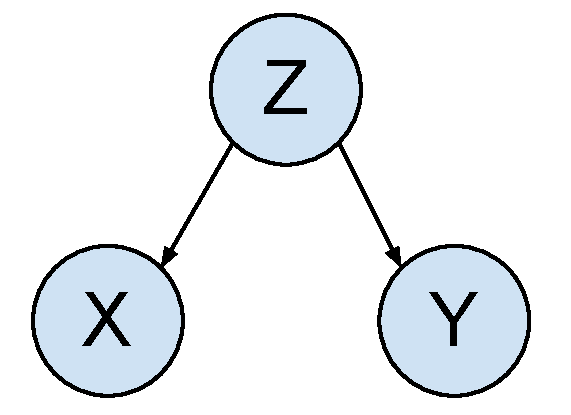
\includegraphics[scale=0.3]{imgs/z2xy}
%		\caption{A common latent cause $Z$}
%		%\label{}	
%	\end{subfigure}
%\end{figure}\pause
%\begin{itemize}
%\item<+-|alert@+> It links causality with probability
%\end{itemize}
%\end{frame}
%\begin{frame}{Functional Causal Model (pearl et al.)} 
%\begin{itemize}[<+->]
%\item A set of variables (factors) $\left\lbrace X_1,\ldots,X_n \right\rbrace$
%\item Directed acyclic graph $\mathcal{G}$ with vertices $\left\lbrace X_1,\ldots,X_n \right\rbrace$
%\item Parents of node $X_i$ in $\mathcal{G}$ are its direct causes
%\item $X_i=f_i(Parents(X_i),\epsilon_i)$, where $\left\lbrace\epsilon_1,\ldots,\epsilon_n\right\rbrace$ are jointly independent noises
%\item The above entails a joint probability distribution $P(X_1,\ldots,X_n)$
%\item Problems are twofold:
%      \begin{enumerate}
%		\item How is the $P$ like?
%		\item Can we recover $\mathcal{G} from P$? 
%	\end{enumerate}
%\item[] \begin{textblock*}{200mm}(0.6\textwidth,-2cm)
%		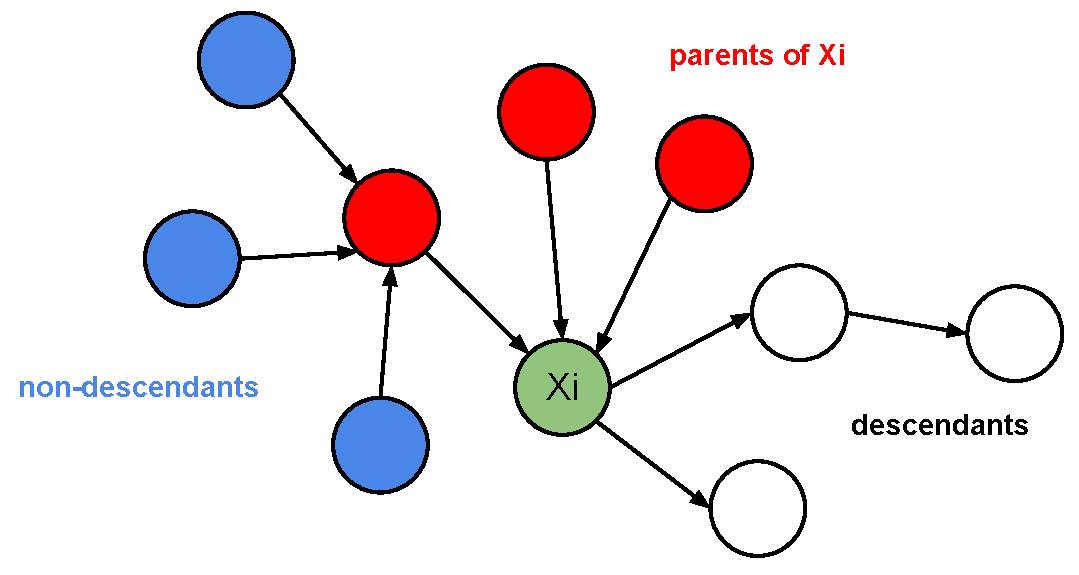
\includegraphics[scale=0.25]{imgs/causalgm}
%	\end{textblock*}
%\end{itemize}
%\end{frame}
%\begin{frame}{Functional Causal Model, ctd.}
%The following are equivalent:
%\begin{itemize}
%\item A functional causal model exists
%\item Local causal Markov condition: $X_i$ is statistically independent of its non-descendants given $X_i$'s parents
%\item Global Causal Markov condition: \textbf{d-separation} characterize the set of independences over all the observables
%\item Factorization: $P(X_1,\ldots,X_n)=\prod_iP(X_i\,|\,Parents(X_i))$
%\end{itemize}
%\end{frame}
%\begin{frame}{Learning causation from Data?}
%\begin{block}{Question}
%Given observational data, can we infer $\mathcal{G}$?
%\end{block}
%\begin{itemize}
%\item \textbf{Simple answer:} impossible without additional information
%\item Possible with interventions (outside force, empirical treatment, etc.)
%\item By conditional independence tests, \textit{Markov equivalence class} containing $\mathcal{G}$ can be learned. \alert{But}, it fails in simplest 2-nodes case.
%\item 2-nodes case can be tackled applying residual dependence test. (see Hoyer et al.)
%\end{itemize}
%\end{frame}
%\begin{frame}{Markov Equivalence Class}
%\textbf{Simplest case with three variables}
%\begin{itemize}
%\item[]<1-> \begin{figure}
%\setcounter{subfigure}{0}
%			\begin{subfigure}[H]{0.4\textwidth}
%			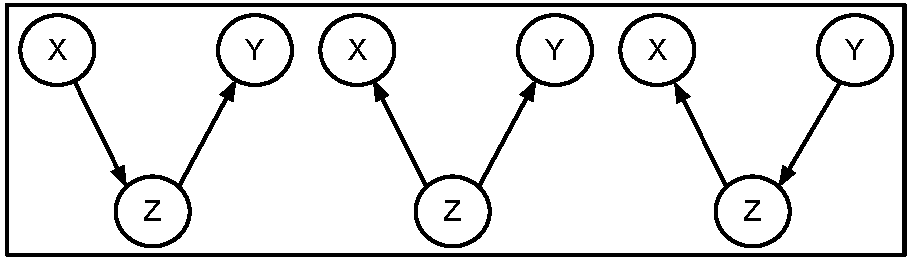
\includegraphics[scale=0.4]{imgs/eqv}
%			\caption{Equivalence}
%			\end{subfigure}\hfill
%			\begin{subfigure}[H]{0.3\textwidth}
%			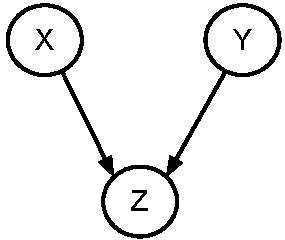
\includegraphics[scale=0.4]{imgs/noneqv}
%			\caption{Non-equivalence}
%			\end{subfigure}
%		\end{figure}
%\item<2-> Samples can be explained by all graphs in equivalence class
%\item<3-> For example:
%\begin{table}
%\centering
%\begin{tabular}{|c|c|}
%\hline
%Equivalence class & Non-equivalence class \\\hline
%$Dep(X,Z\,|\,\emptyset)$ & $Dep(X,Z\,|\,\emptyset)$\\\hline
%$Dep(Y,Z\,|\,\emptyset)$ & $Dep(Y,Z\,|\,\emptyset)$\\\hline
%$Dep(X,Y\,|\,\emptyset)$ & \alert{$Ind(X,Y\,|\,\emptyset)$}\\\hline
%$Ind(X,Y\,|\,Z)$ & \alert{$Dep(X,Y\,|\,Z)$}\\\hline
%\end{tabular}
%\end{table}	
%\end{itemize}
%\end{frame}
\section{Indicative Support Vector Clustering}
\subsection{Reweights of penalties}
\begin{frame}{Punishments are not fair}
Recall the penalty term...
\[
\min \left(R^2 + C\sum \xi_i\right)
\]
The higher the punishment value $C$ is...
\begin{itemize}
\item the lower the summation $\sum \xi_i$ is
\item the less likely $\xi_i > 0$
\item the less likely data points $\left\lbrace x_i\right\rbrace$ run out of sphere
\item the less outliers are allowed!
\end{itemize}
\pause
\vskip20pt 
\color{red} We see that, for all the outliers, penalty is the same $C$.
\end{frame}
\begin{frame}{Reweight the penalties}
Now we treat data points individually instead of equivalently penalizing all the input data with a constant $C$...
\begin{align}
\min \left(R^2 + \sum c_i\xi_i\right) \nonumber
\end{align}  
The larger the penalty $c_i$ is, the less possible the point $x_i$ would be driven away from the hypersphere, and vice versa. 
\pause
\vskip30pt
\begin{center}
\large
\color{blue} Full control over each point!
\end{center}
\end{frame}
\subsection{Integrate indicative information}
\begin{frame}{Assumption}
\begin{block}{ }
Anomalies are the patterns found to behave distinctly from the normal patterns, and similarly behaving instances are more likely hosted in the same cluster. 
\end{block}
\end{frame}
\begin{frame}{User given labels}
Suppose part of user feedback is available, 
\begin{center}
\begin{align*}
\mathcal{X^+}=&\left\lbrace \left( x_l, y_l) \,|\,  x_l \in \mathcal{X}, y_l=1 \right)\right\rbrace\\
\mathcal{X^-}=&\left\lbrace \left( x_r, y_r) \,|\, x_r \in \mathcal{X}, y_r=-1\right)\right\rbrace\\
&l, r \in \left\lbrace 1,\ldots ,N\right\rbrace
\end{align*}
\end{center}
$\mathcal{X^+}$ is set of outliers indicated by users, and $\mathcal{X}$ a set of normal samples.
\end{frame}
\begin{frame}{Impact function}
The closer to the indicated data, the more likely they belong to the same set (normal/outlier)
\begin{figure}
\centering
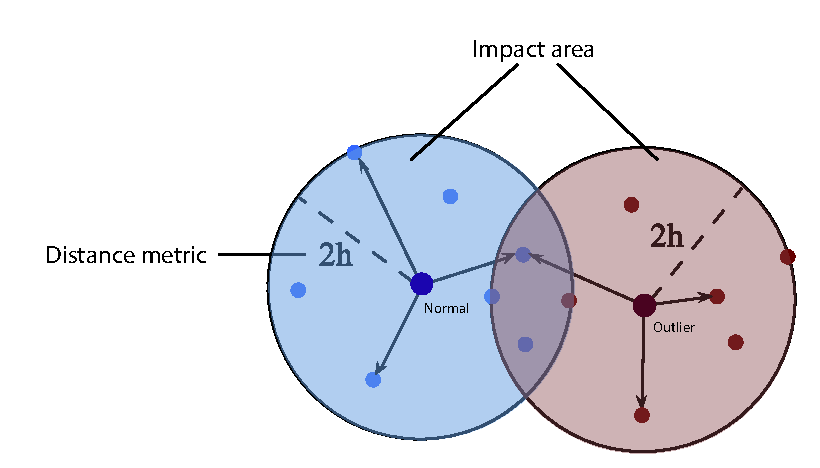
\includegraphics[scale=0.5]{imgs/indicative2.pdf}
\end{figure}
\vskip10pt
\pause
\color{blue}So, the penalties can be reweighed by distances to the given labeled data points.
\end{frame}

\subsection{Observations}
\begin{frame}{We observed}
Points near the given outliers $\mathcal{X^+}$
\begin{itemize}
\item Penalties $c_j$ are small
\item More likely to be repelled
\item Impact on cluster center $g$ is small
\end{itemize}
\pause
Points near the given normals $\mathcal{X^-}$
\begin{itemize}
\item Penalties $c_j$ are big
\item More likely to be enclosed into the ball
\item Impact on cluster center $g$ is larger
\end{itemize}
\pause
Leads to...
\begin{itemize}
\item Robustness
\item Reliable outlier detection
\item Better clustering results
\item More compact bound
\end{itemize}
\end{frame}
%\begin{frame}{Statistical Implication}
%\begin{block}{Reichenbach's \textit{Common Cause Principle}}
%If $X$ and $Y$ are correlated, then either $X$ causes $Y$ or $Y$ causes $X$ or they share a latent common cause $Z$.
%\end{block}
%\begin{figure}
%\setcounter{subfigure}{0}
%	\centering
%	\begin{subfigure}[H]{0.3\textwidth}
%		\centering
%		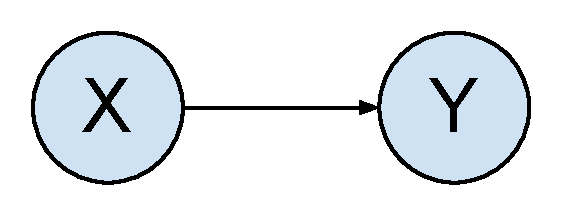
\includegraphics[scale=0.3]{imgs/x2y}
%		\caption{$X$ causes $Y$}
%		%\label{}	
%	\end{subfigure}
%	\begin{subfigure}[H]{0.3\textwidth}
%		\centering
%		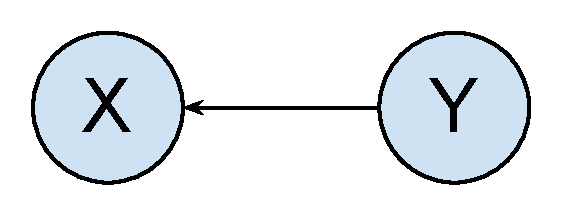
\includegraphics[scale=0.3]{imgs/y2x}
%		\caption{$Y$ causes $X$}
%		%\label{}	
%	\end{subfigure}
%	\begin{subfigure}[H]{0.3\textwidth}
%		\centering
%		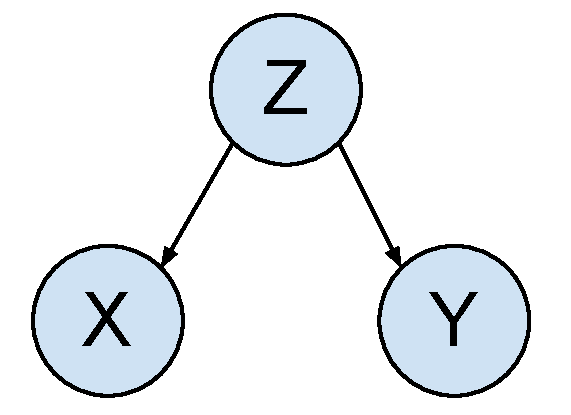
\includegraphics[scale=0.3]{imgs/z2xy}
%		\caption{A common latent cause $Z$}
%		%\label{}	
%	\end{subfigure}
%\end{figure}\pause
%\begin{itemize}
%\item<+-|alert@+> It links causality with probability
%\end{itemize}
%\end{frame}
%\begin{frame}{Functional Causal Model (pearl et al.)} 
%\begin{itemize}[<+->]
%\item A set of variables (factors) $\left\lbrace X_1,\ldots,X_n \right\rbrace$
%\item Directed acyclic graph $\mathcal{G}$ with vertices $\left\lbrace X_1,\ldots,X_n \right\rbrace$
%\item Parents of node $X_i$ in $\mathcal{G}$ are its direct causes
%\item $X_i=f_i(Parents(X_i),\epsilon_i)$, where $\left\lbrace\epsilon_1,\ldots,\epsilon_n\right\rbrace$ are jointly independent noises
%\item The above entails a joint probability distribution $P(X_1,\ldots,X_n)$
%\item Problems are twofold:
%      \begin{enumerate}
%		\item How is the $P$ like?
%		\item Can we recover $\mathcal{G} from P$? 
%	\end{enumerate}
%\item[] \begin{textblock*}{200mm}(0.6\textwidth,-2cm)
%		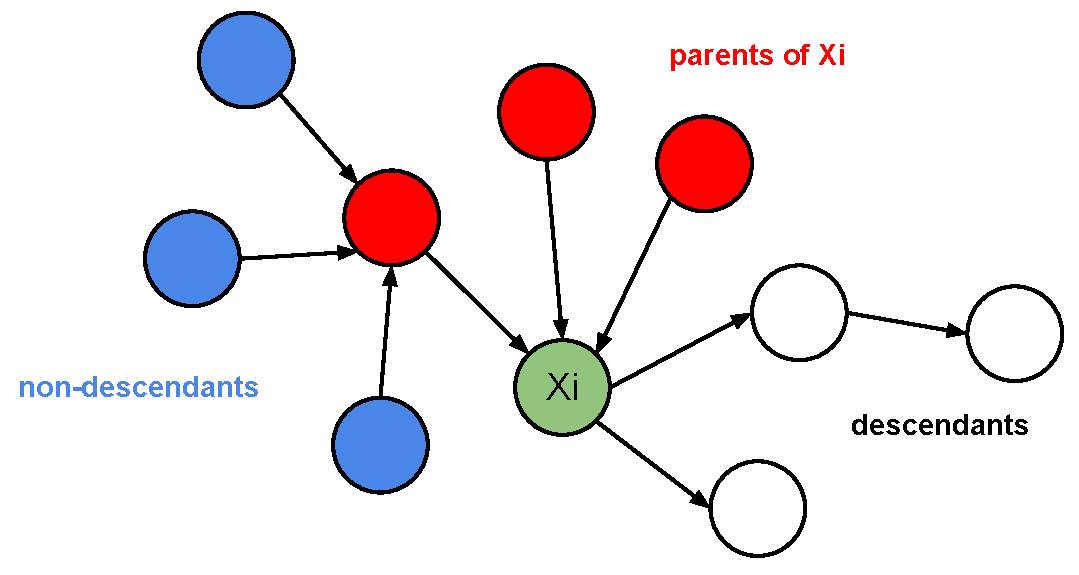
\includegraphics[scale=0.25]{imgs/causalgm}
%	\end{textblock*}
%\end{itemize}
%\end{frame}
%\begin{frame}{Functional Causal Model, ctd.}
%The following are equivalent:
%\begin{itemize}
%\item A functional causal model exists
%\item Local causal Markov condition: $X_i$ is statistically independent of its non-descendants given $X_i$'s parents
%\item Global Causal Markov condition: \textbf{d-separation} characterize the set of independences over all the observables
%\item Factorization: $P(X_1,\ldots,X_n)=\prod_iP(X_i\,|\,Parents(X_i))$
%\end{itemize}
%\end{frame}
%\begin{frame}{Learning causation from Data?}
%\begin{block}{Question}
%Given observational data, can we infer $\mathcal{G}$?
%\end{block}
%\begin{itemize}
%\item \textbf{Simple answer:} impossible without additional information
%\item Possible with interventions (outside force, empirical treatment, etc.)
%\item By conditional independence tests, \textit{Markov equivalence class} containing $\mathcal{G}$ can be learned. \alert{But}, it fails in simplest 2-nodes case.
%\item 2-nodes case can be tackled applying residual dependence test. (see Hoyer et al.)
%\end{itemize}
%\end{frame}
%\begin{frame}{Markov Equivalence Class}
%\textbf{Simplest case with three variables}
%\begin{itemize}
%\item[]<1-> \begin{figure}
%\setcounter{subfigure}{0}
%			\begin{subfigure}[H]{0.4\textwidth}
%			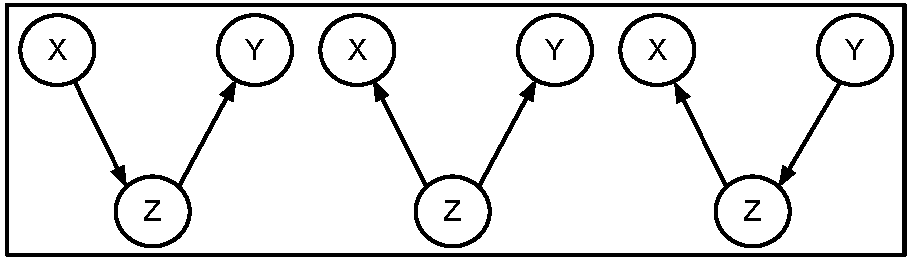
\includegraphics[scale=0.4]{imgs/eqv}
%			\caption{Equivalence}
%			\end{subfigure}\hfill
%			\begin{subfigure}[H]{0.3\textwidth}
%			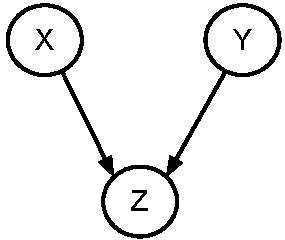
\includegraphics[scale=0.4]{imgs/noneqv}
%			\caption{Non-equivalence}
%			\end{subfigure}
%		\end{figure}
%\item<2-> Samples can be explained by all graphs in equivalence class
%\item<3-> For example:
%\begin{table}
%\centering
%\begin{tabular}{|c|c|}
%\hline
%Equivalence class & Non-equivalence class \\\hline
%$Dep(X,Z\,|\,\emptyset)$ & $Dep(X,Z\,|\,\emptyset)$\\\hline
%$Dep(Y,Z\,|\,\emptyset)$ & $Dep(Y,Z\,|\,\emptyset)$\\\hline
%$Dep(X,Y\,|\,\emptyset)$ & \alert{$Ind(X,Y\,|\,\emptyset)$}\\\hline
%$Ind(X,Y\,|\,Z)$ & \alert{$Dep(X,Y\,|\,Z)$}\\\hline
%\end{tabular}
%\end{table}	
%\end{itemize}
%\end{frame}
\section{Experimental results}
\subsection{Synthetic data set experiments}
\begin{frame}{On synthetic data set}
Setup
\begin{itemize}
\item Two normal classes data: 250 samples of each
\item A ring-like Outlier data set: 150 samples
\item Given different sets of data labels
\end{itemize}
\end{frame}
\begin{frame}{Results I}
Given 5 outliers / 15 outliers...
\begin{figure}
\centering
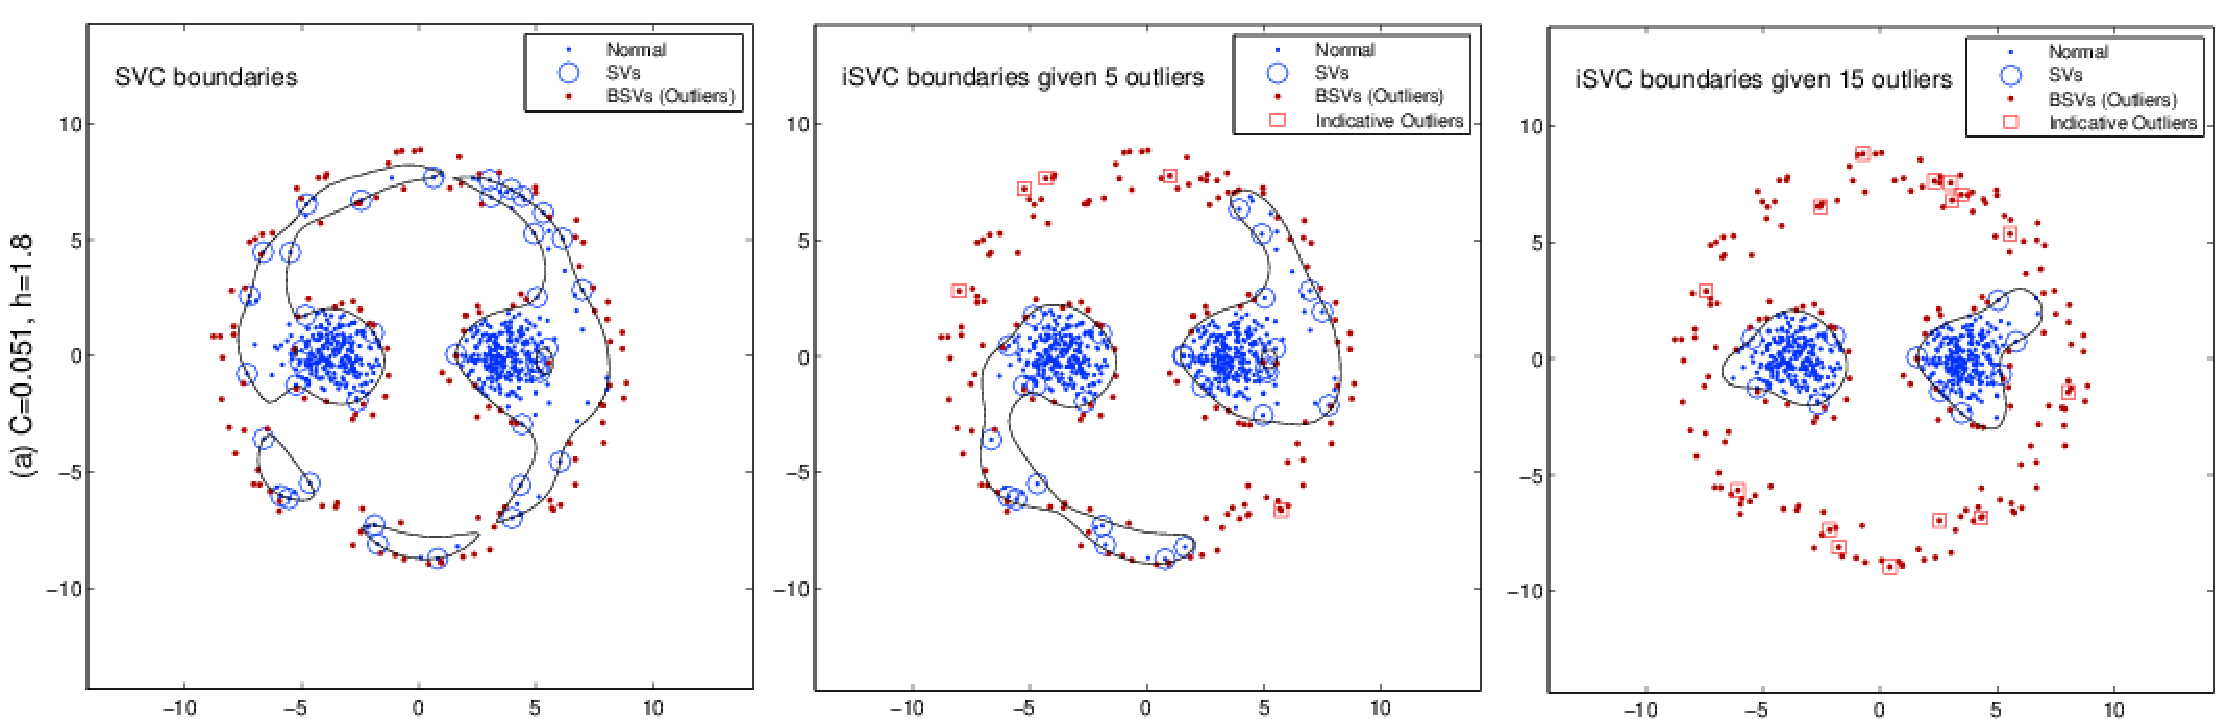
\includegraphics[scale=0.28]{imgs/syn_01_01.pdf}\\
%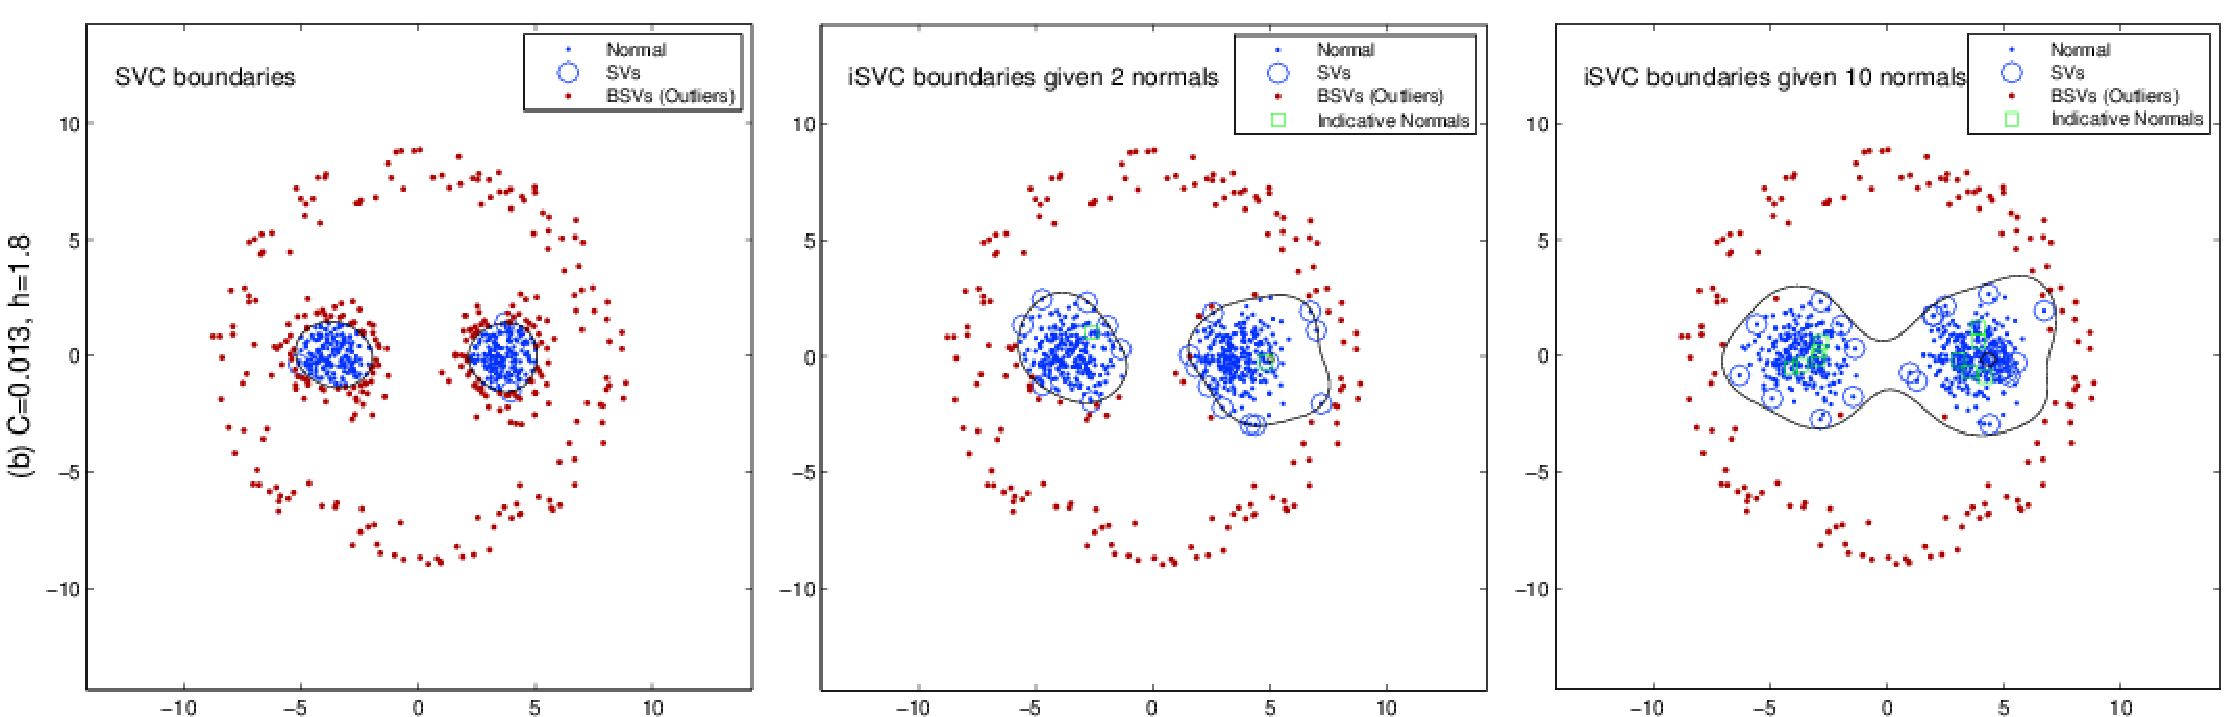
\includegraphics[scale=0.5\textwidth]{imgs/syn_01_02}\\
%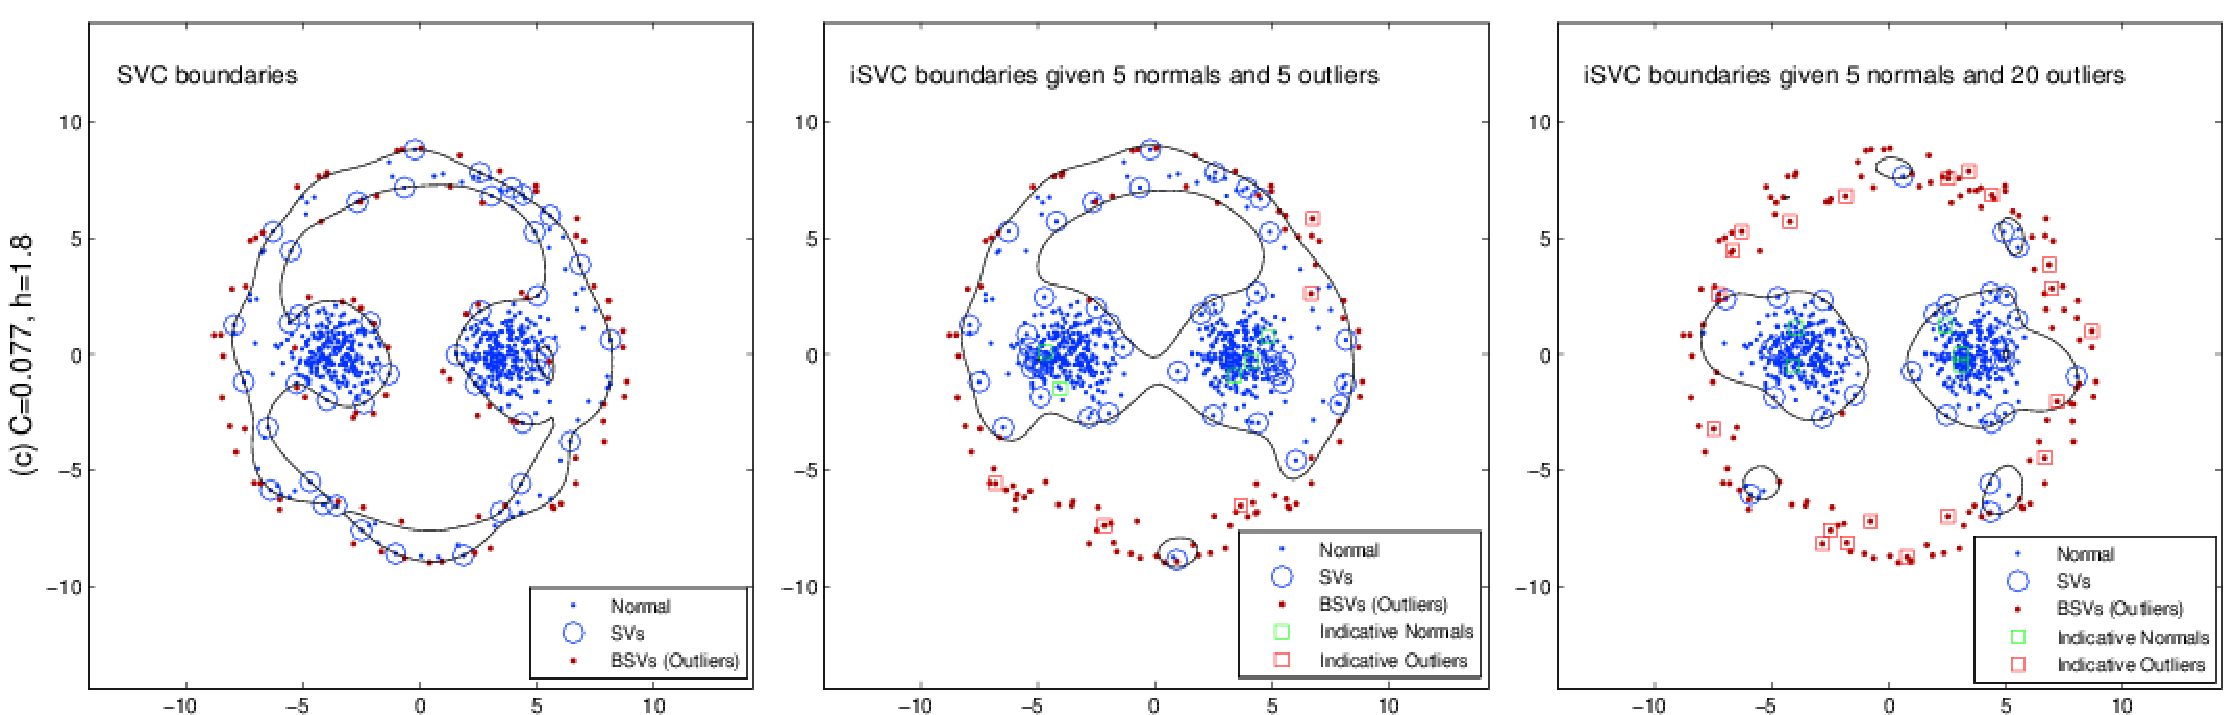
\includegraphics[scale=0.5\textwidth]{imgs/syn_01_03}
\end{figure}
\end{frame}
\begin{frame}{Results II}
Given 2 Normals / 10 Normals...
\begin{figure}
\centering
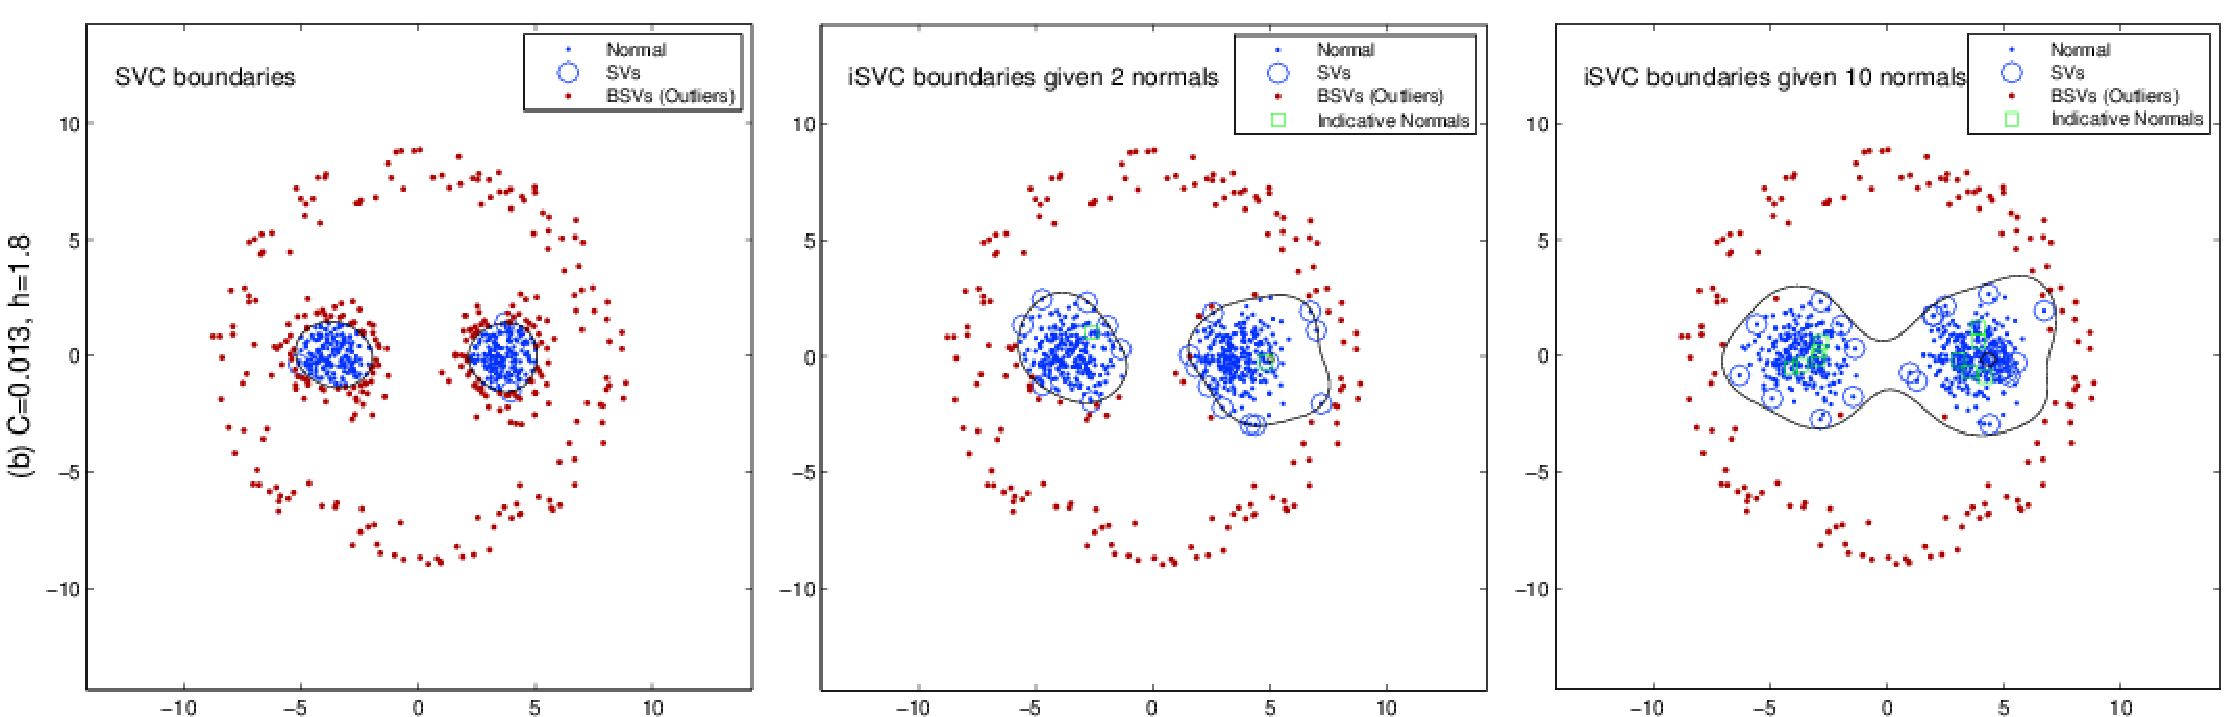
\includegraphics[scale=0.28]{imgs/syn_01_02.pdf}\\
%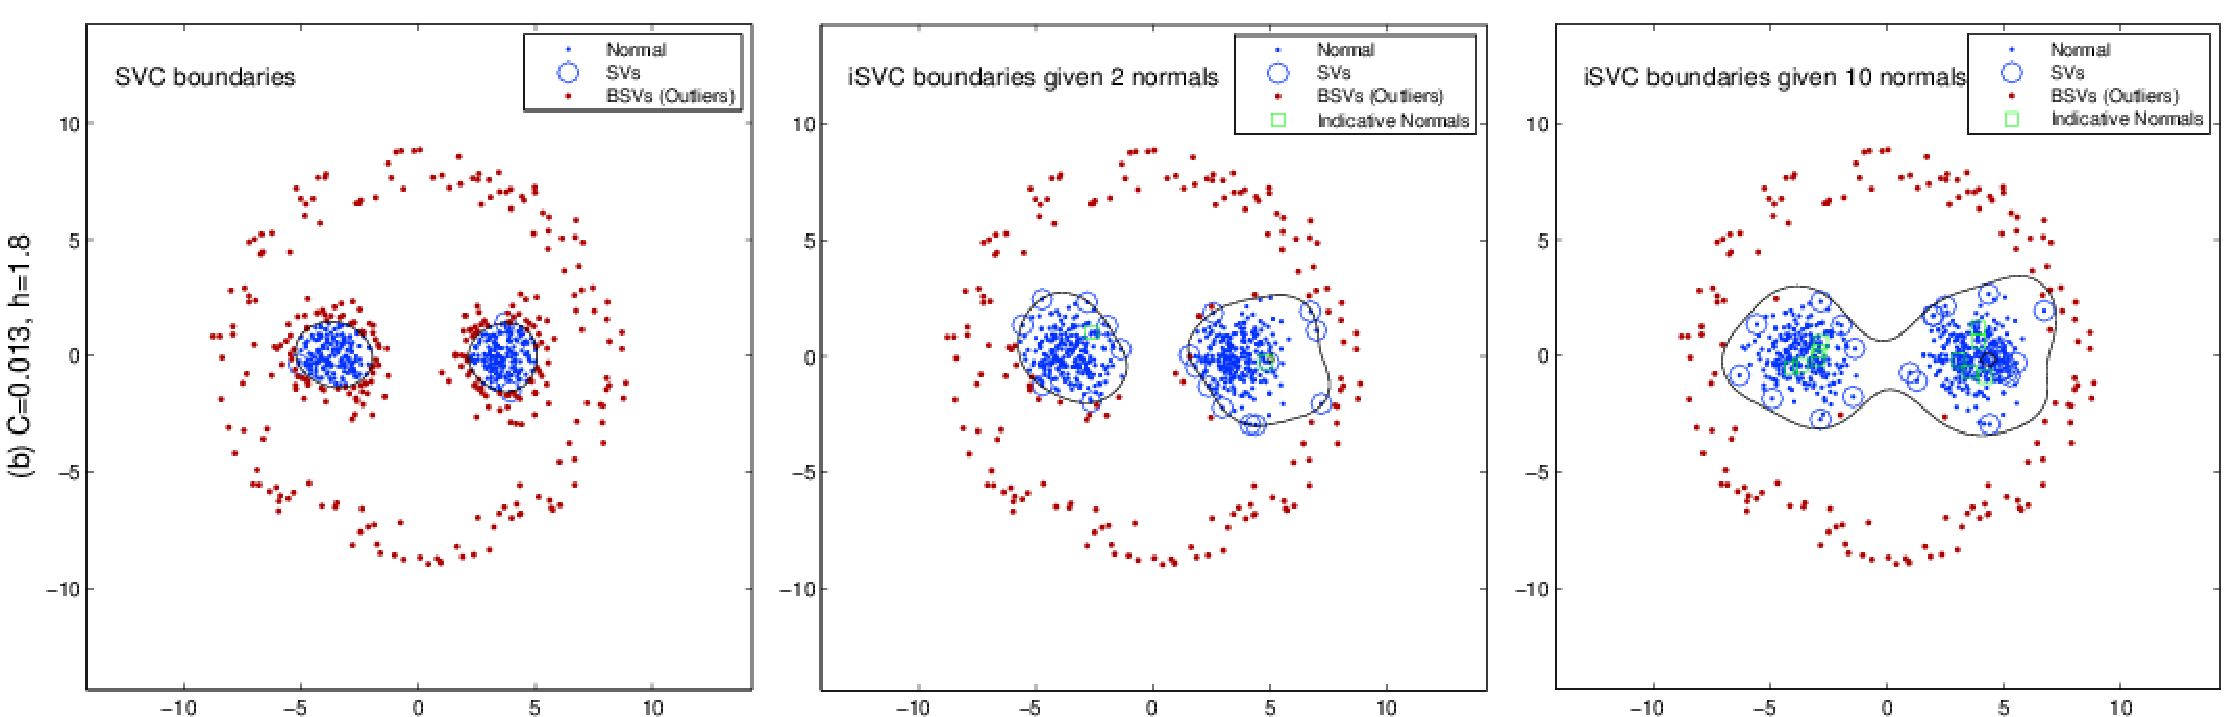
\includegraphics[scale=0.5\textwidth]{imgs/syn_01_02}\\
%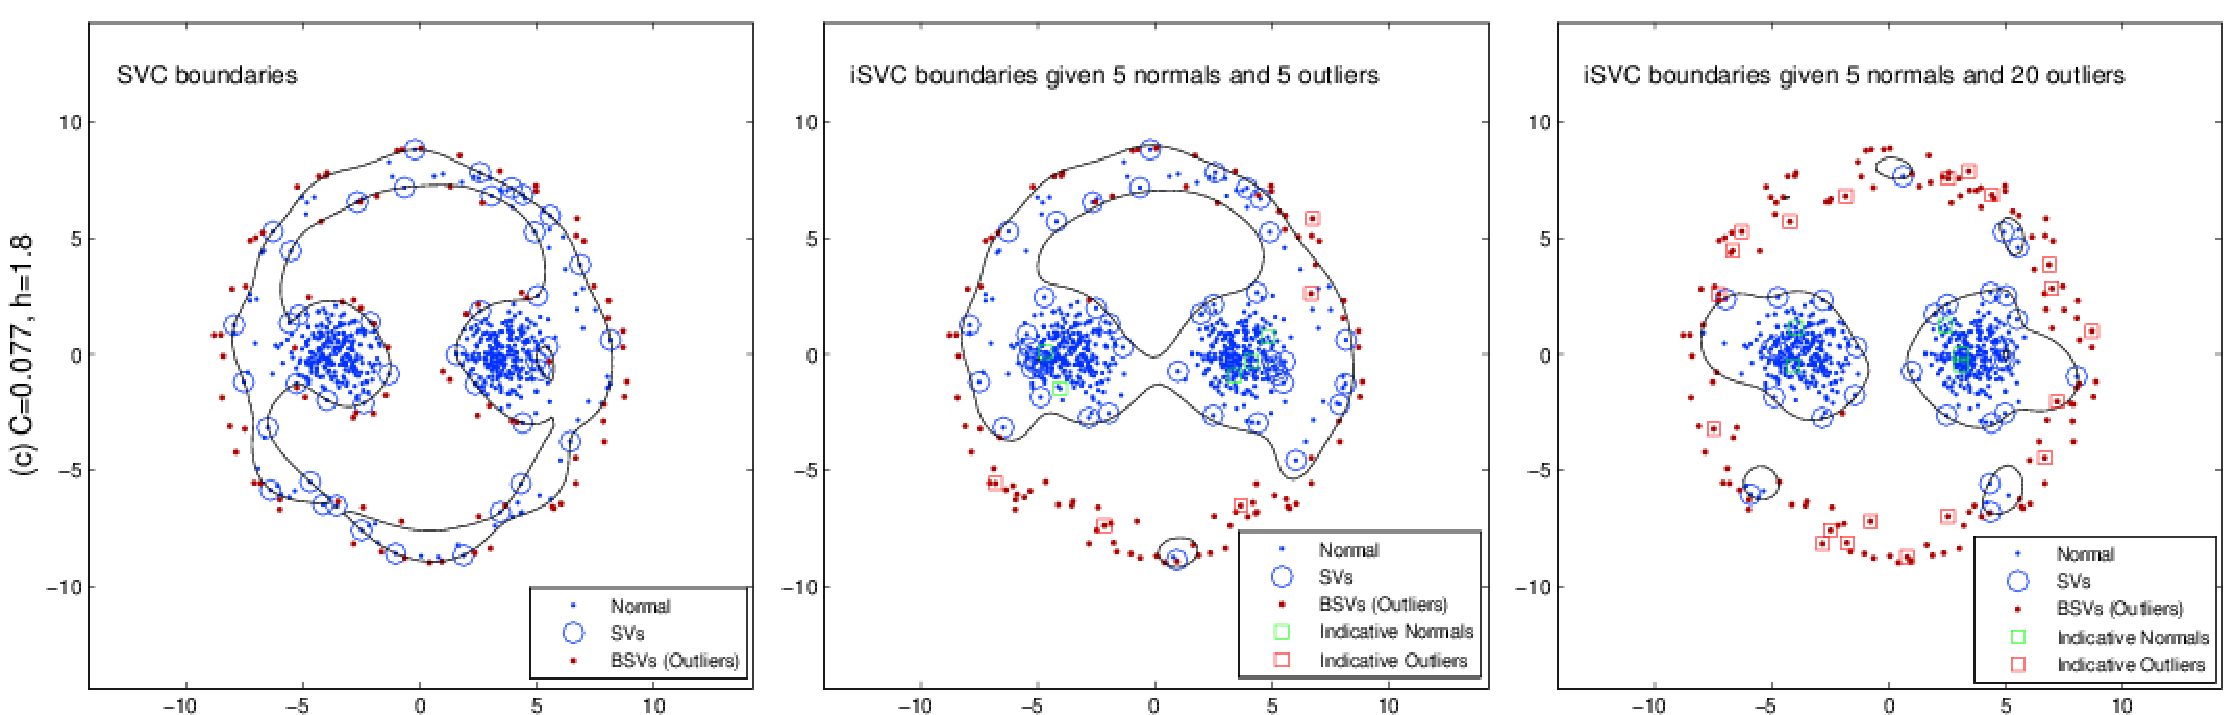
\includegraphics[scale=0.5\textwidth]{imgs/syn_01_03}
\end{figure}
\end{frame}
\begin{frame}{Results III}
Given 5 Normals and 5 Outliers / 5 Normals and 20 outliers...
\begin{figure}
\centering
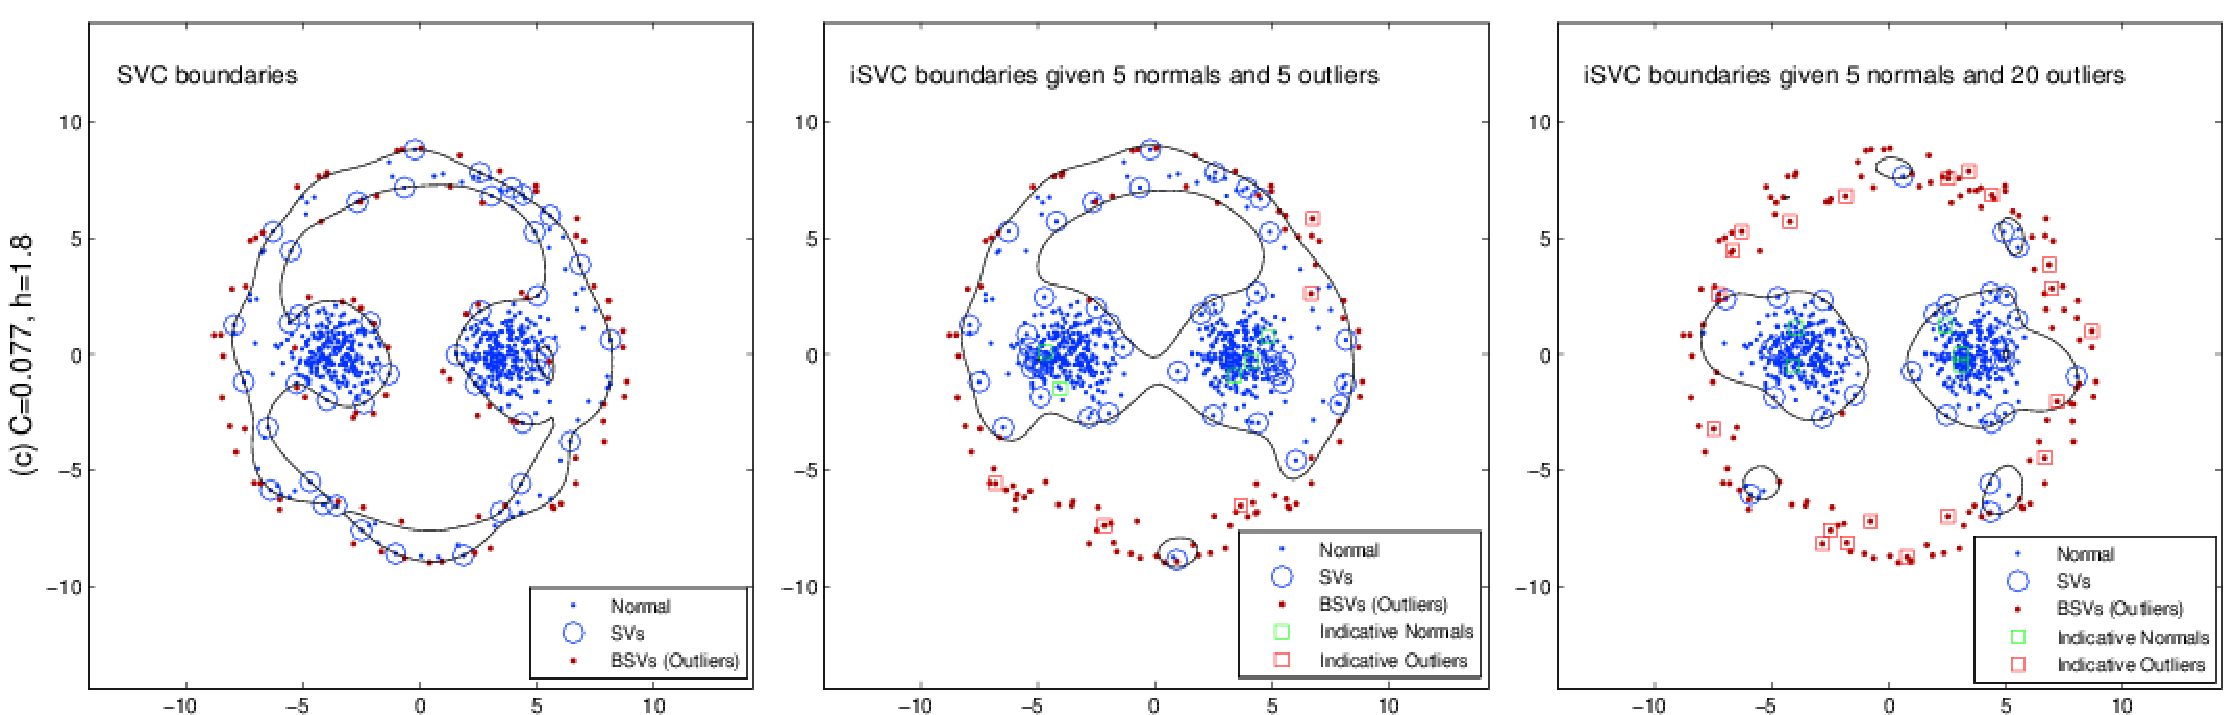
\includegraphics[scale=0.28]{imgs/syn_01_03.pdf}\\
%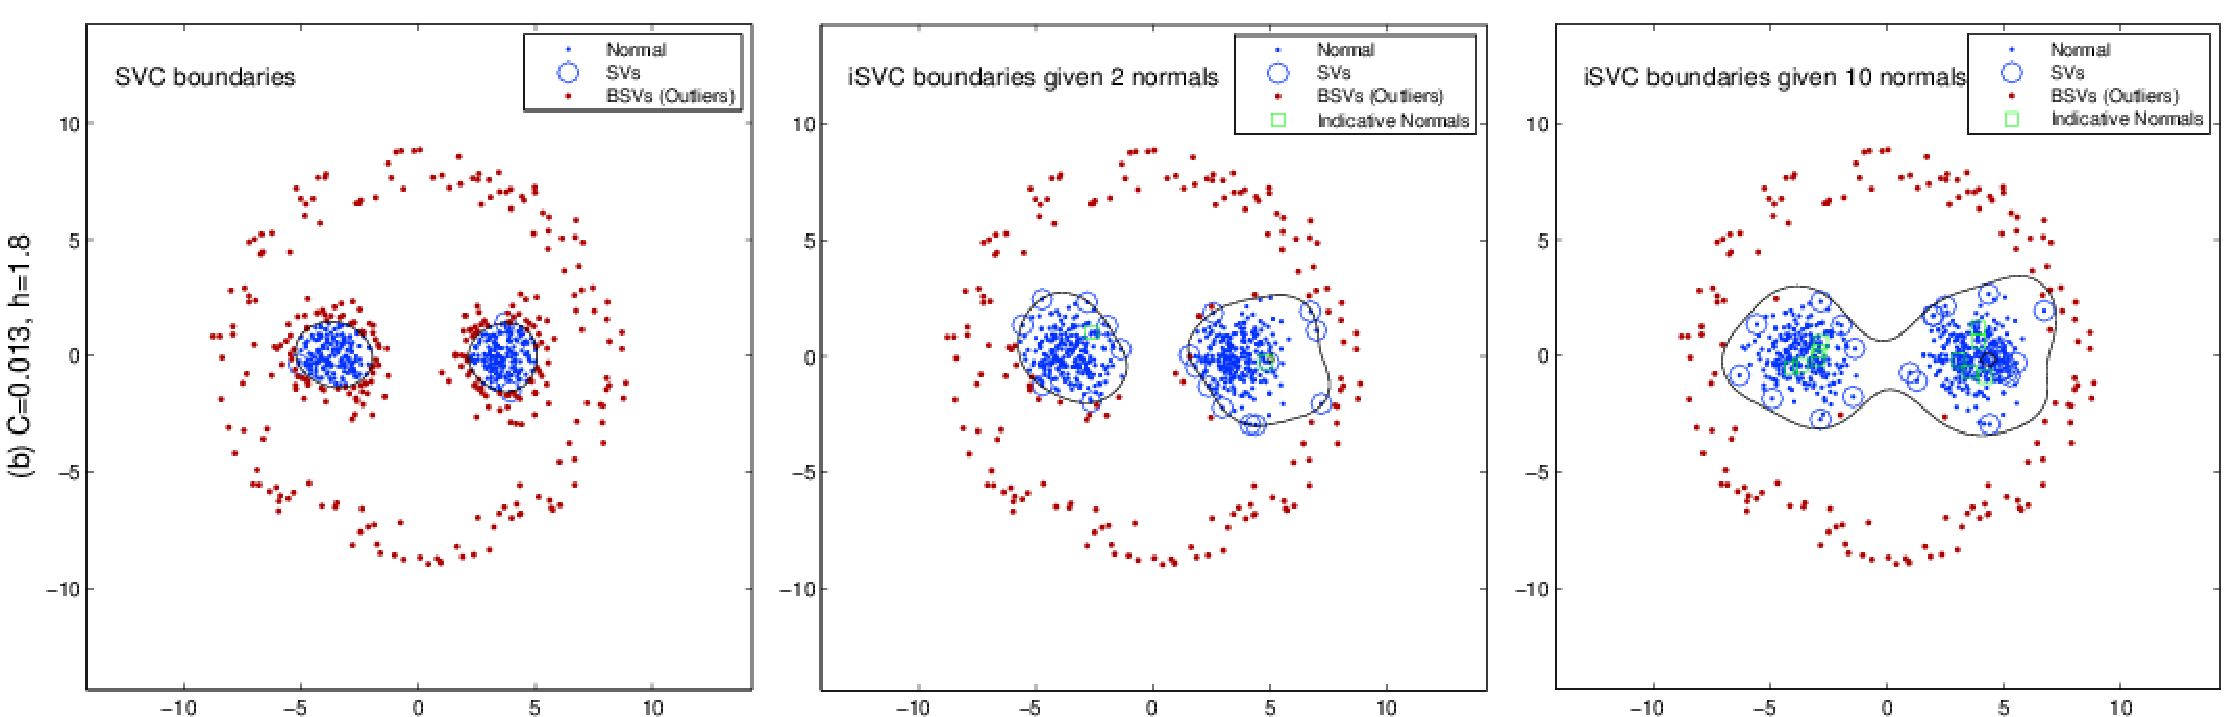
\includegraphics[scale=0.5\textwidth]{imgs/syn_01_02}\\
%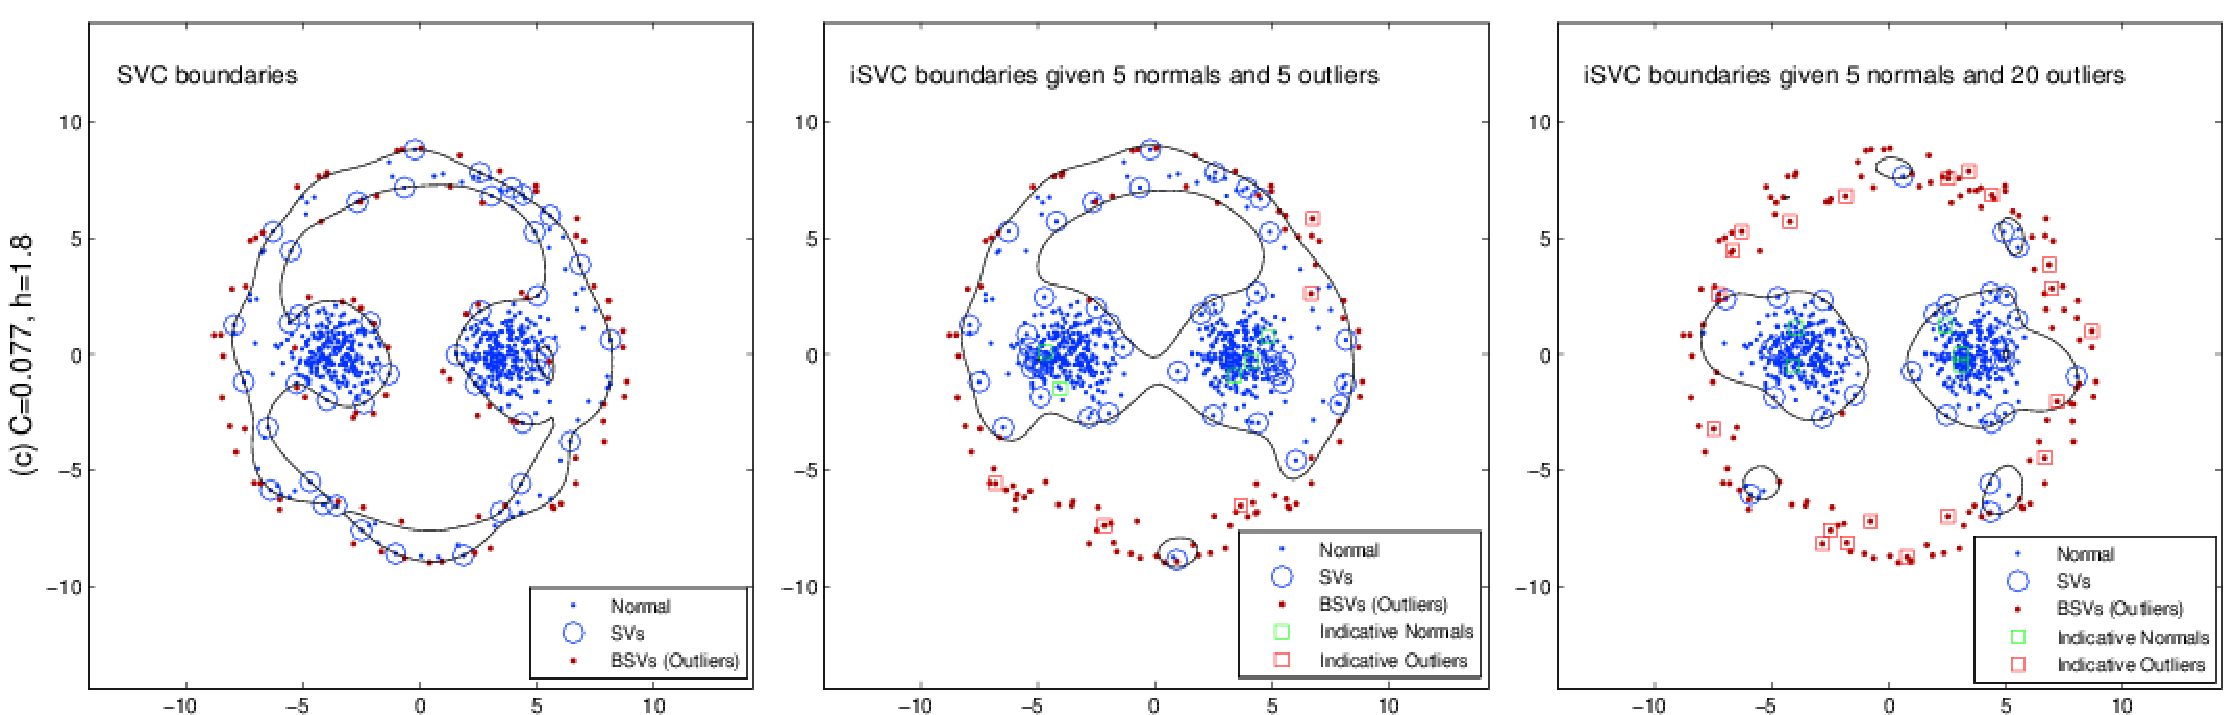
\includegraphics[scale=0.5\textwidth]{imgs/syn_01_03}
\end{figure}
\end{frame}

\subsection{Real-world data set experiments}
\begin{frame}{On digits recognition data set}
\begin{itemize}
\item MINST digit images data set
\item Digits {2,6,9}, 150 images of each
\item 100 digit {0} tampered manually as outliers
\end{itemize}
\begin{figure}
\centering
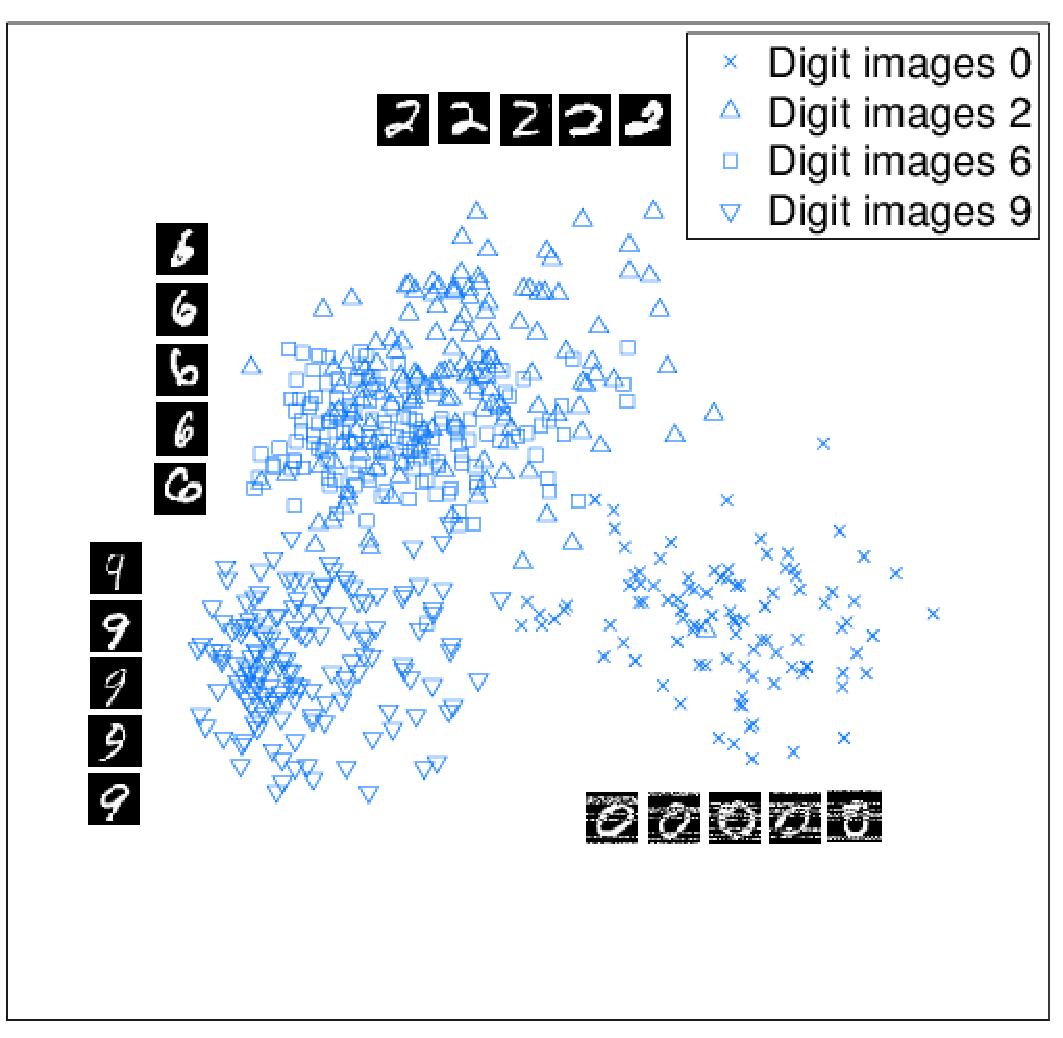
\includegraphics[scale=0.198]{imgs/real_01_01.pdf}
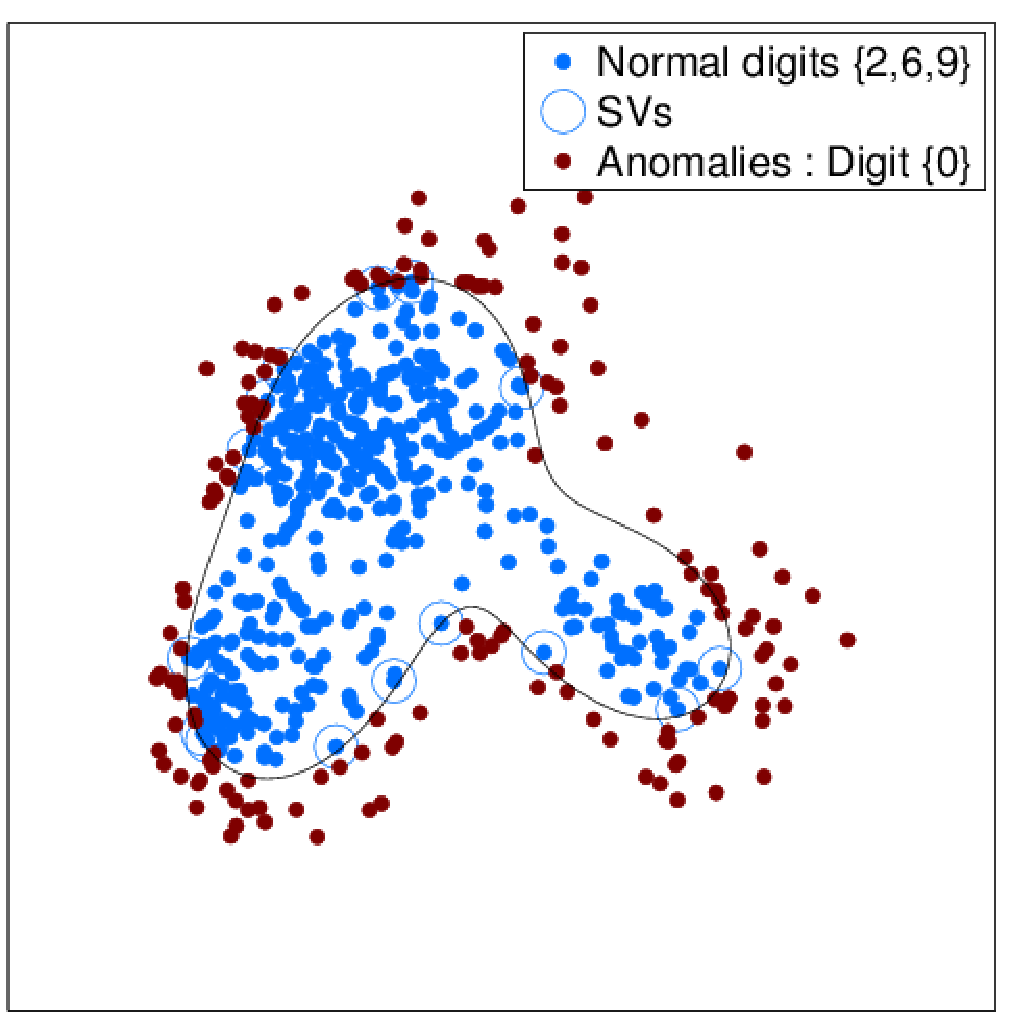
\includegraphics[scale=0.2]{imgs/real_01_02.pdf}
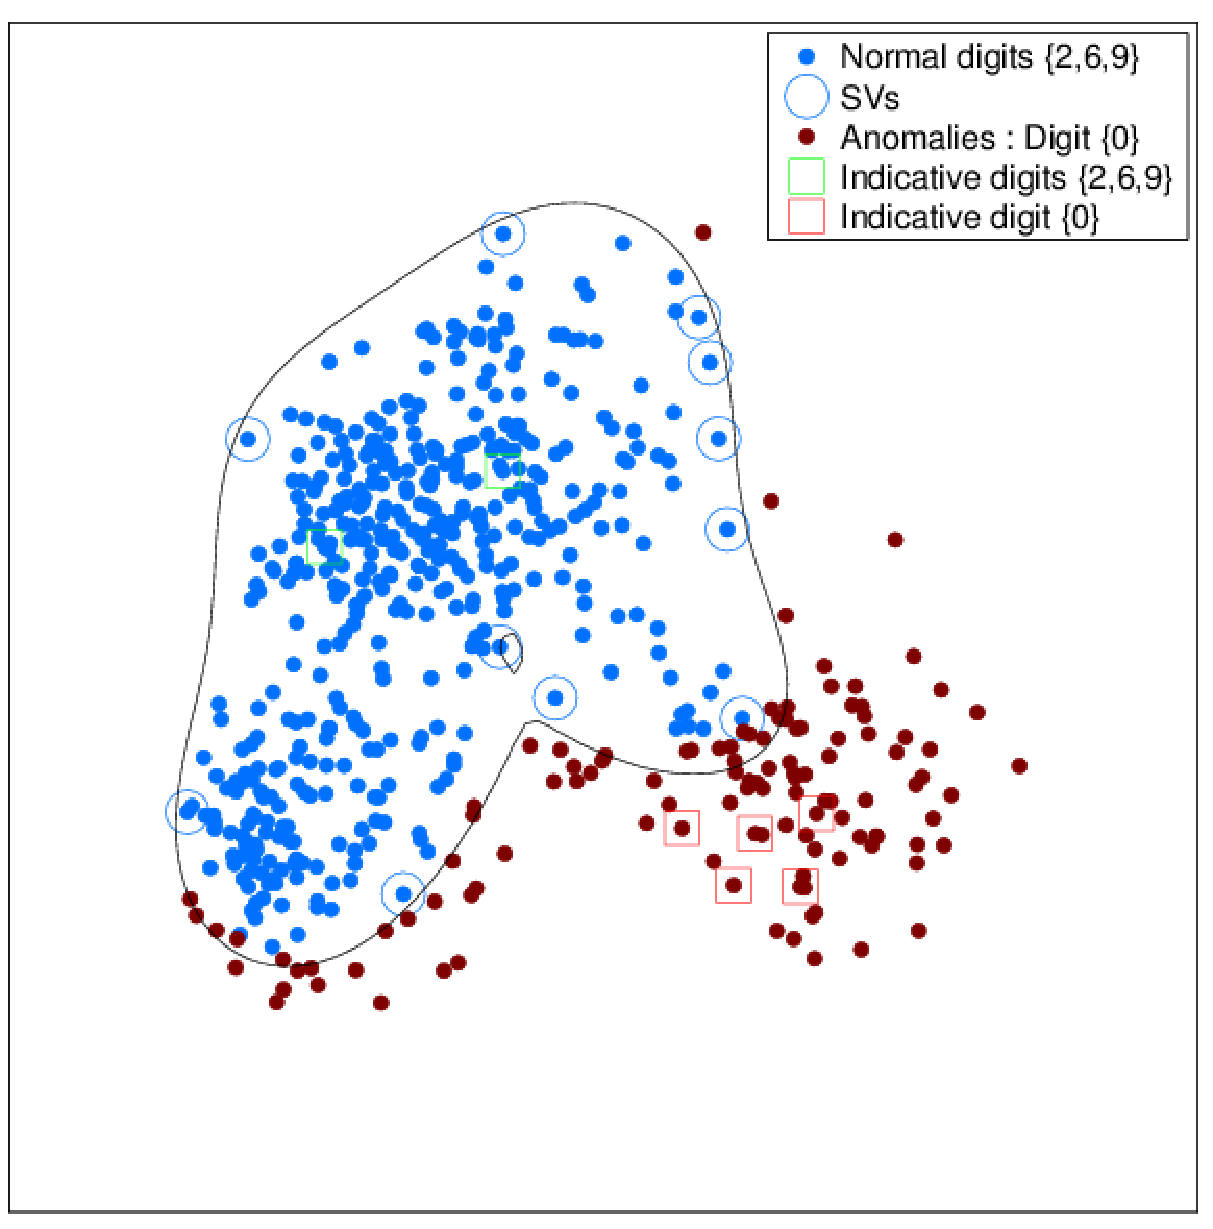
\includegraphics[scale=0.167]{imgs/real_01_03.pdf}
\end{figure}
\end{frame}
\begin{frame}{Numerical evaluation}
\begin{figure}
\centering
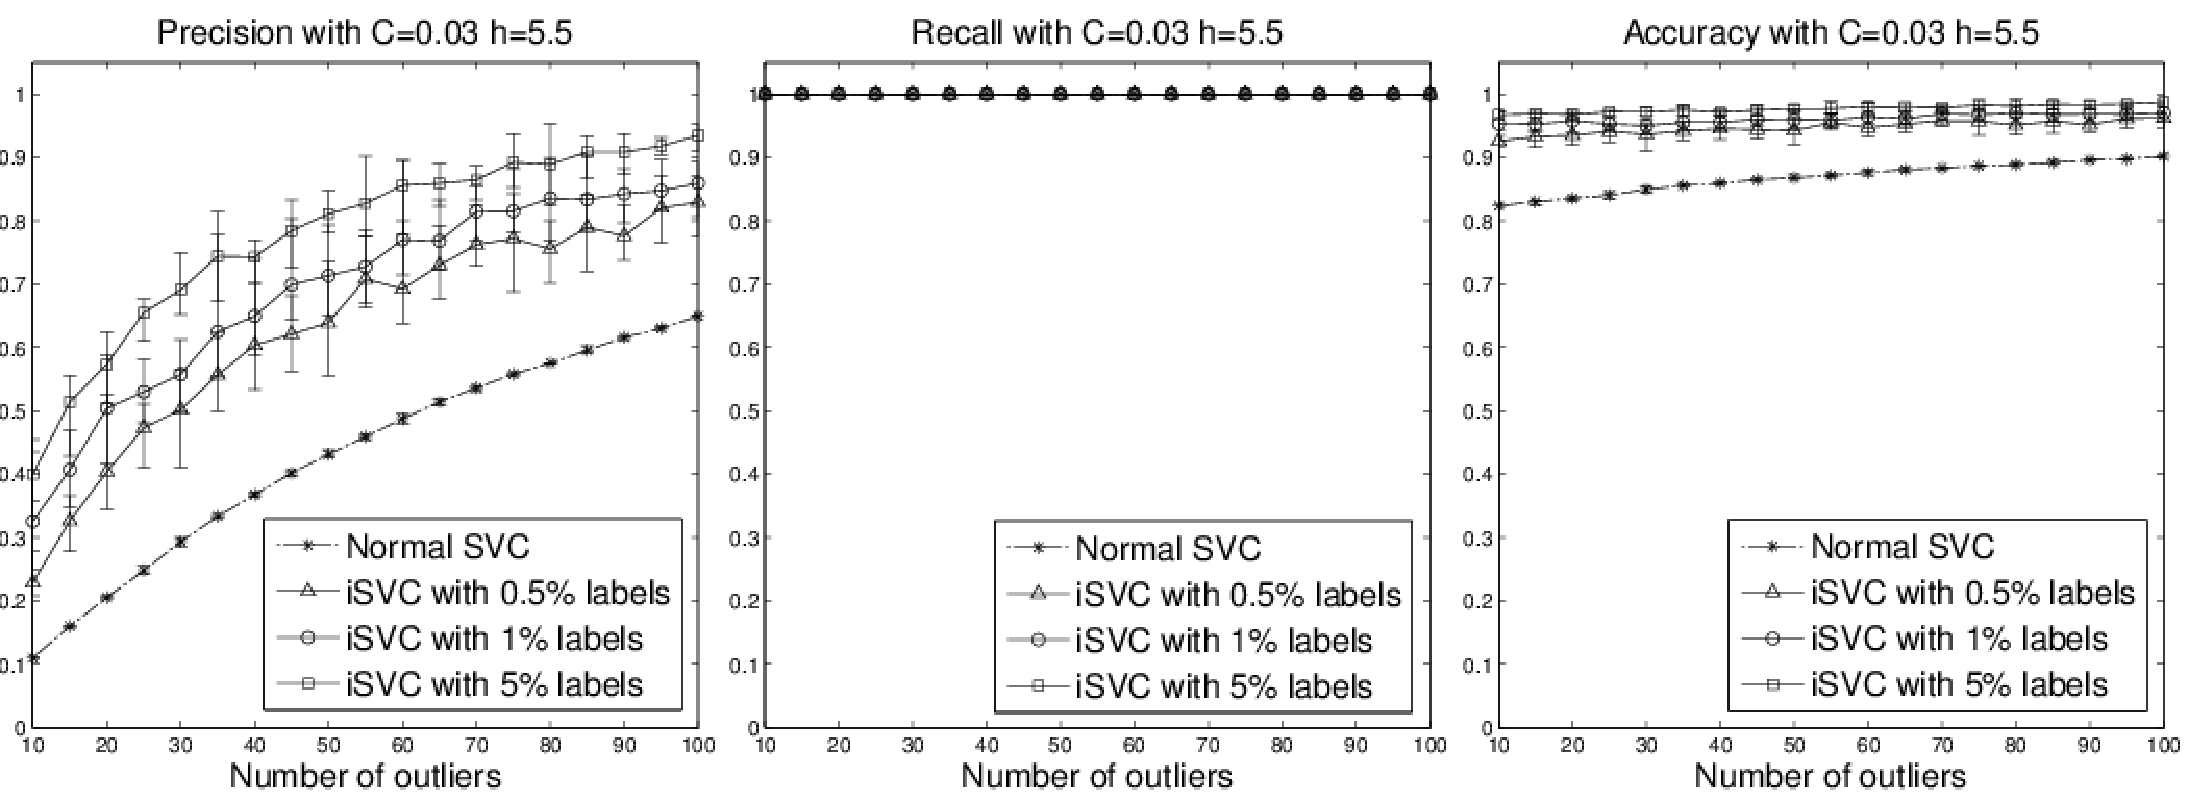
\includegraphics[scale=0.25]{imgs/real_02.pdf}\\
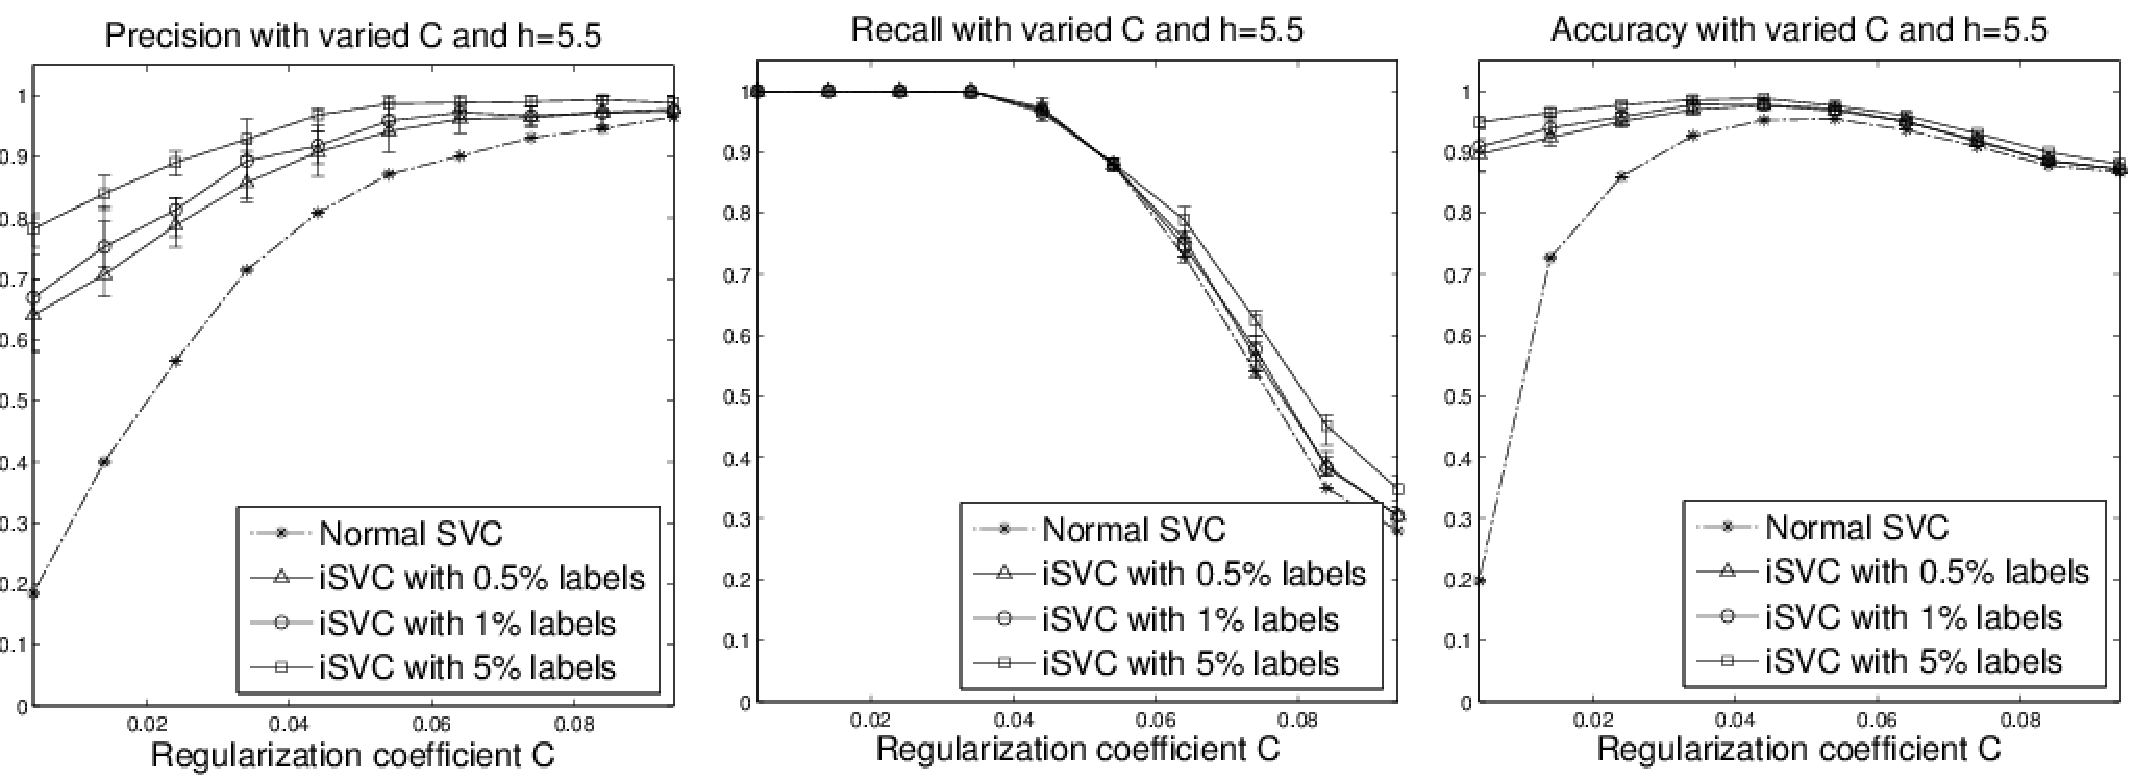
\includegraphics[scale=0.25]{imgs/real_03.pdf}
\end{figure}
\end{frame}
\begin{frame}{On the WDBC data set}
\begin{itemize}
\item Wisconsin Diagnostic Breast Cancer (WDBC) data set
\item 569 samples, out of which 212 are malignant and 357 are benign
\item Test it against semi-supervised fast linear SVM given various labels
\end{itemize}
\end{frame}
\begin{frame}{Results}
\begin{table}[!t]
\small
\setlength{\tabcolsep}{10pt}
% increase table row spacing, adjust to taste
\renewcommand{\arraystretch}{1.3}
% if using array.sty, it might be a good idea to tweak the value of
% \extrarowheight as needed to properly center the text within the cells
%\caption{Empirical results on the WDBC data set given different proportions of sample labels.}
\label{tbl:real_03}
\centering
% Some packages, such as MDW tools, offer better commands for making tables
% than the plain LaTeX2e tabular which is used here.
\begin{tabular}{|c||c|c|c|c|}
\hline
& \multicolumn{4}{c|}{\textbf{WDBC data set with $\mathbf{h=0.9, C=0.001}$}}\\
\cline{2-5}
& Accuracy & $F_1$-measure & FPR & FNR \\
\hline
\textit{SVC} & $63.4\%$ & $50.5\%$ & $28.6\%$ &$50\%$ \\\hline
& \multicolumn{4}{c|}{$5\%$ \textit{positive} and $0\%$ \textit{negative} labels}\\
\hline
\textit{iSVC} & $\mathbf{90.5\%}$ & $\mathbf{87.0\%}$ & $\mathbf{6.4\%}$ &$14.6\%$ \\\hline
\textit{S3VM} & $39.2\%$ & $55.0\%$ & $96.9\%$ &$\mathbf{0\%}$ \\\hline
& \multicolumn{4}{c|}{$0\%$ \textit{positive} and $5\%$ \textit{negative} labels}\\
\hline
\textit{iSVC} & $\mathbf{89.8\%}$ & $\mathbf{87.7\%}$ & $14.8\%$ &$2.4\%$ \\\hline
\textit{S3VM} & $64.9\%$ & $10.7\%$ & $\mathbf{0\%}$ &$94.3\%$ \\\hline
& \multicolumn{4}{c|}{$5\%$ \textit{positive} and $5\%$ \textit{negative} labels}\\
\hline
\textit{iSVC} & $\mathbf{92.3\%}$ & $\mathbf{89.8\%}$ & $\mathbf{7.0\%}$ &$8.9\%$ \\\hline
\textit{S3VM} & $88.4\%$ & $86.3\%$ & $17.4\%$ &$\mathbf{1.9\%}$ \\\hline
& \multicolumn{4}{c|}{$10\%$ \textit{positive} and $10\%$ \textit{negative} labels} \\
\hline
\textit{iSVC} & $\mathbf{93.9\%}$ & $\mathbf{91.9\%}$ & $\mathbf{6.4\%}$ &$5.6\%$ \\\hline
\textit{S3VM} & $92.4\%$ & $90.6\%$ & $10.4\%$ &$\mathbf{2.8\%}$ \\\hline
\end{tabular}
\end{table}
\end{frame}
%\begin{frame}{Statistical Implication}
%\begin{block}{Reichenbach's \textit{Common Cause Principle}}
%If $X$ and $Y$ are correlated, then either $X$ causes $Y$ or $Y$ causes $X$ or they share a latent common cause $Z$.
%\end{block}
%\begin{figure}
%\setcounter{subfigure}{0}
%	\centering
%	\begin{subfigure}[H]{0.3\textwidth}
%		\centering
%		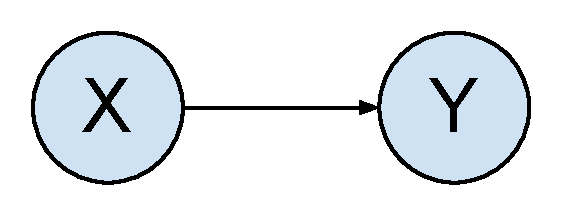
\includegraphics[scale=0.3]{imgs/x2y}
%		\caption{$X$ causes $Y$}
%		%\label{}	
%	\end{subfigure}
%	\begin{subfigure}[H]{0.3\textwidth}
%		\centering
%		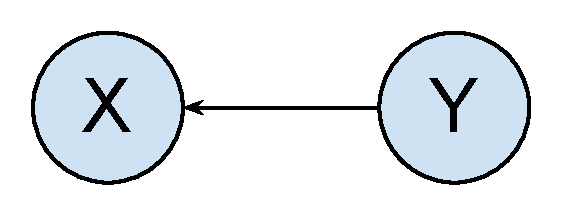
\includegraphics[scale=0.3]{imgs/y2x}
%		\caption{$Y$ causes $X$}
%		%\label{}	
%	\end{subfigure}
%	\begin{subfigure}[H]{0.3\textwidth}
%		\centering
%		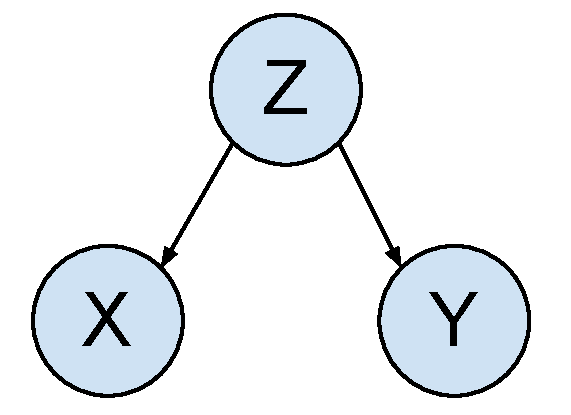
\includegraphics[scale=0.3]{imgs/z2xy}
%		\caption{A common latent cause $Z$}
%		%\label{}	
%	\end{subfigure}
%\end{figure}\pause
%\begin{itemize}
%\item<+-|alert@+> It links causality with probability
%\end{itemize}
%\end{frame}
%\begin{frame}{Functional Causal Model (pearl et al.)} 
%\begin{itemize}[<+->]
%\item A set of variables (factors) $\left\lbrace X_1,\ldots,X_n \right\rbrace$
%\item Directed acyclic graph $\mathcal{G}$ with vertices $\left\lbrace X_1,\ldots,X_n \right\rbrace$
%\item Parents of node $X_i$ in $\mathcal{G}$ are its direct causes
%\item $X_i=f_i(Parents(X_i),\epsilon_i)$, where $\left\lbrace\epsilon_1,\ldots,\epsilon_n\right\rbrace$ are jointly independent noises
%\item The above entails a joint probability distribution $P(X_1,\ldots,X_n)$
%\item Problems are twofold:
%      \begin{enumerate}
%		\item How is the $P$ like?
%		\item Can we recover $\mathcal{G} from P$? 
%	\end{enumerate}
%\item[] \begin{textblock*}{200mm}(0.6\textwidth,-2cm)
%		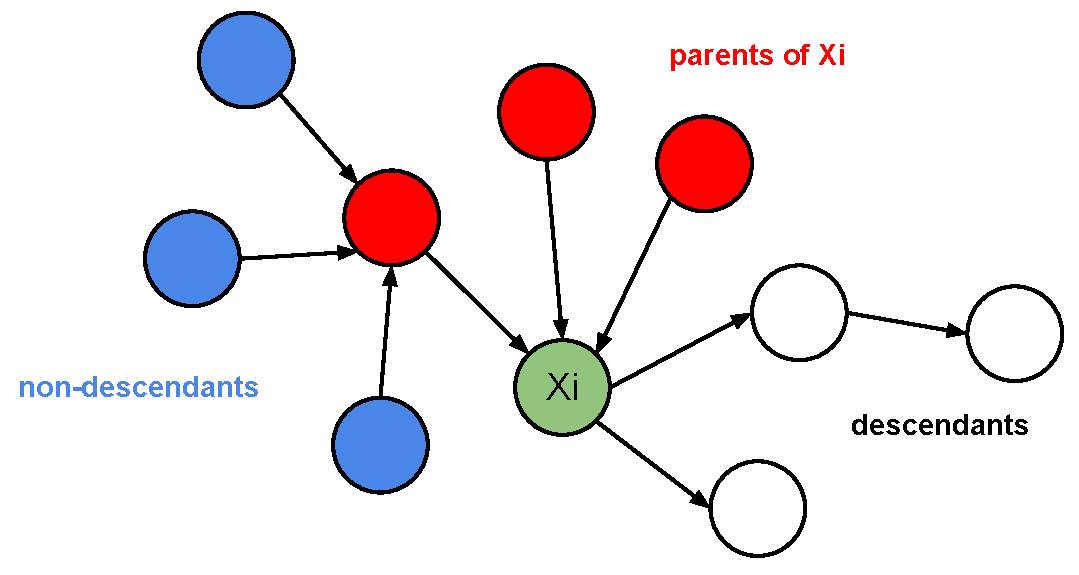
\includegraphics[scale=0.25]{imgs/causalgm}
%	\end{textblock*}
%\end{itemize}
%\end{frame}
%\begin{frame}{Functional Causal Model, ctd.}
%The following are equivalent:
%\begin{itemize}
%\item A functional causal model exists
%\item Local causal Markov condition: $X_i$ is statistically independent of its non-descendants given $X_i$'s parents
%\item Global Causal Markov condition: \textbf{d-separation} characterize the set of independences over all the observables
%\item Factorization: $P(X_1,\ldots,X_n)=\prod_iP(X_i\,|\,Parents(X_i))$
%\end{itemize}
%\end{frame}
%\begin{frame}{Learning causation from Data?}
%\begin{block}{Question}
%Given observational data, can we infer $\mathcal{G}$?
%\end{block}
%\begin{itemize}
%\item \textbf{Simple answer:} impossible without additional information
%\item Possible with interventions (outside force, empirical treatment, etc.)
%\item By conditional independence tests, \textit{Markov equivalence class} containing $\mathcal{G}$ can be learned. \alert{But}, it fails in simplest 2-nodes case.
%\item 2-nodes case can be tackled applying residual dependence test. (see Hoyer et al.)
%\end{itemize}
%\end{frame}
%\begin{frame}{Markov Equivalence Class}
%\textbf{Simplest case with three variables}
%\begin{itemize}
%\item[]<1-> \begin{figure}
%\setcounter{subfigure}{0}
%			\begin{subfigure}[H]{0.4\textwidth}
%			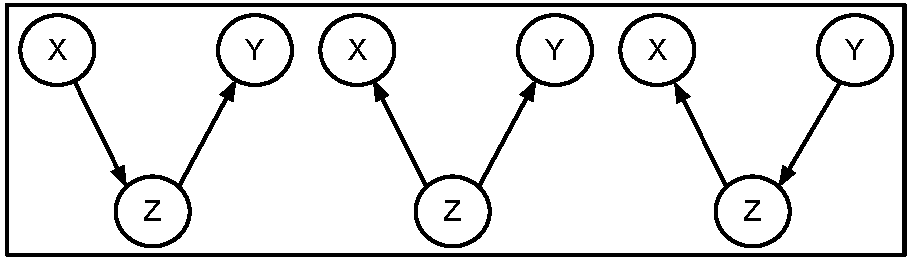
\includegraphics[scale=0.4]{imgs/eqv}
%			\caption{Equivalence}
%			\end{subfigure}\hfill
%			\begin{subfigure}[H]{0.3\textwidth}
%			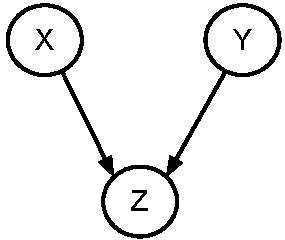
\includegraphics[scale=0.4]{imgs/noneqv}
%			\caption{Non-equivalence}
%			\end{subfigure}
%		\end{figure}
%\item<2-> Samples can be explained by all graphs in equivalence class
%\item<3-> For example:
%\begin{table}
%\centering
%\begin{tabular}{|c|c|}
%\hline
%Equivalence class & Non-equivalence class \\\hline
%$Dep(X,Z\,|\,\emptyset)$ & $Dep(X,Z\,|\,\emptyset)$\\\hline
%$Dep(Y,Z\,|\,\emptyset)$ & $Dep(Y,Z\,|\,\emptyset)$\\\hline
%$Dep(X,Y\,|\,\emptyset)$ & \alert{$Ind(X,Y\,|\,\emptyset)$}\\\hline
%$Ind(X,Y\,|\,Z)$ & \alert{$Dep(X,Y\,|\,Z)$}\\\hline
%\end{tabular}
%\end{table}	
%\end{itemize}
%\end{frame}
\section{Conclusion}
\begin{frame}{Conclusion}
We have
\begin{itemize}
\item More robust clustering method
\item Outliers are more reliable
\item User's feedback can be integrated
\end{itemize}
Future work
\begin{itemize}
\item More sophisticated impact function
\item Online mode of iSVC
\item Automation of model selection
\end{itemize}
\end{frame}
\section{References}
\begin{frame}{References}
\begin{thebibliography}{99}
\bibitem{Boas}Huang Xiao, Claudia Eckert. Indicative support vector clustering and its application on anomaly detection.  \textit{In IEEE 12th International Conference on Machine Learning and Applications }, Dec. 2013.
\end{thebibliography}
\end{frame}
\begin{frame}{Appendix}
Given a data set of $N$ points $\left\lbrace x_i \right\rbrace_{i=1}^N \subseteq \mathcal{X}$, 
defining a non-linear feature mapping $\Phi$ from $\mathcal{X}$ to a higher dimensional Hilbert space $\mathcal{H}$,

\begin{align}
\label{eq:svc1}
&\min R^2 + \sum c_i\xi_i\\		
\text{subject to}\quad &  \| \Phi(x_j) - g\|^2 \leq R^2 + \xi_j,\; \forall j \nonumber \\
& \xi_j \geq 0 \nonumber
\end{align} 
Introducing the Lagrangian
\begin{align}
\label{eq:svc2}
L=R^2&-\sum_j\left(R^2+\xi_j-\|\Phi(x_j)-g\|^2\right)\beta_j\nonumber\\
     &-\sum\xi_j\mu_j+\sum c_i\xi_j,
\end{align}
$\beta_j\geq 0$ and $\mu_j\geq 0$ are Lagrange multipliers, $c_i$ is the regularization constant.
\end{frame}
\begin{frame}
Two supervised data sets are indicated by users, 
\begin{align*}
\mathcal{X^+}=&\left\lbrace \left( x_l, y_l) \,|\,  x_l \in \mathcal{X}, y_l=1 \right)\right\rbrace\\
\mathcal{X^-}=&\left\lbrace \left( x_r, y_r) \,|\, x_r \in \mathcal{X}, y_r=-1\right)\right\rbrace\\
&l, r \in \left\lbrace 1,\ldots ,N\right\rbrace
\end{align*}
where $\mathcal{X^+}$ is the outlier set, and $\mathcal{X^-}$ is normal set.
\end{frame}
\begin{frame}
An impact function $f$ is defined in the input space $\mathcal{X}$ given $\mathcal{X^+}$ and $\mathcal{X^-}$.  
\begin{gather}
f\left(x_i\right) = \frac{\sum_{x_l\in \mathcal{X^+}}K\left(x_l, x_i\right)}{\sum_l\mathbf{1^+}\left(x_l,x_i\right)} + 
\frac{\sum_{x_r\in \mathcal{X^-}}K\left(x_r, x_i\right)}{\sum_l\mathbf{1^-}\left(x_r,x_i\right)}
\end{gather}
where the kernel function is taken as a similarity measurement, note that
\[
K(x, x_i) = \exp\left(\frac{\| x - x_i \|^2}{-2h^2}\right)
\]
And $\mathbf{1^+}$ and $\mathbf{1^-}$ are both indicator functions defined as
\begin{align*}
\mathbf{1^+}(x_l, x_i)= &
     \begin{cases}
     	1 & \quad \| x_l - x_i \| \leq 2h\\
     	0 & \quad \text{otherwise}
     \end{cases}\\
\mathbf{1^-}(x_r, x_i)=&
     \begin{cases}
     	-1 & \quad \| x_r - x_i \| \leq 2h\\
     	0 & \quad \text{otherwise}
     \end{cases}     
\end{align*}
\end{frame}
\begin{frame}
The regularization weights $c_j$ can be computed
\begin{align}
c_j = \begin{cases}
c_0 \cdot \frac{1-f\left(x_j\right)}{1-\exp\left(-2\right)} + \frac{1}{N}\cdot \frac{f\left(x_j\right) - \exp\left(-2\right)}{1-\exp\left(-2\right)} & \text{if}\quad f\left(x_j\right) > 0\\
c_0 \cdot \frac{1-\left|f\left(x_j\right)\right|}{1-\exp\left(-2\right)} + \frac{\left|f\left(x_j\right)\right| - \exp\left(-2\right)}{1-\exp\left(-2\right)} & \text{if}\quad f\left(x_j\right) < 0
\end{cases}
\end{align}
where $c_0$ is the initial value of $c_j$ and $N$ is the sample size.
\end{frame}
\begin{frame}
Now setting the derivative of the Lagrange $L$ to zero, we have:
\begin{align}
\sum\beta_j=1\\
g=\sum\beta_j\Phi(x_j)\\
\beta_j=c_j-\mu_j
\end{align}  
The KKT conditions again require that
\begin{gather}
\xi_j\mu_j=0\\
\left(R^2+\xi_j-\|\Phi(x_j)-g\|^2\right)\beta_j=0
\end{gather} 
\end{frame}
\begin{frame}
Eliminating the variables $R$, $g$, and $u_j$, the Wolf dual form is obtained, where $\beta_j$ are the only variables.
\begin{gather}
W=\sum_j\Phi(x_j)^2\beta_j-\sum_{i,j}\beta_i\beta_j\Phi(x_i)\cdot\Phi(x_j)\\
\text{subject to}\quad 0\leq\beta_j\leq c_j, \; j=1,\ldots,N. 
\end{gather}
Solve the dual problem, we have found $\left\lbrace \beta_j \right\rbrace$.
\end{frame}
%\begin{frame}{Statistical Implication}
%\begin{block}{Reichenbach's \textit{Common Cause Principle}}
%If $X$ and $Y$ are correlated, then either $X$ causes $Y$ or $Y$ causes $X$ or they share a latent common cause $Z$.
%\end{block}
%\begin{figure}
%\setcounter{subfigure}{0}
%	\centering
%	\begin{subfigure}[H]{0.3\textwidth}
%		\centering
%		\includegraphics[scale=0.3]{imgs/x2y}
%		\caption{$X$ causes $Y$}
%		%\label{}	
%	\end{subfigure}
%	\begin{subfigure}[H]{0.3\textwidth}
%		\centering
%		\includegraphics[scale=0.3]{imgs/y2x}
%		\caption{$Y$ causes $X$}
%		%\label{}	
%	\end{subfigure}
%	\begin{subfigure}[H]{0.3\textwidth}
%		\centering
%		\includegraphics[scale=0.3]{imgs/z2xy}
%		\caption{A common latent cause $Z$}
%		%\label{}	
%	\end{subfigure}
%\end{figure}\pause
%\begin{itemize}
%\item<+-|alert@+> It links causality with probability
%\end{itemize}
%\end{frame}
%\begin{frame}{Functional Causal Model (pearl et al.)} 
%\begin{itemize}[<+->]
%\item A set of variables (factors) $\left\lbrace X_1,\ldots,X_n \right\rbrace$
%\item Directed acyclic graph $\mathcal{G}$ with vertices $\left\lbrace X_1,\ldots,X_n \right\rbrace$
%\item Parents of node $X_i$ in $\mathcal{G}$ are its direct causes
%\item $X_i=f_i(Parents(X_i),\epsilon_i)$, where $\left\lbrace\epsilon_1,\ldots,\epsilon_n\right\rbrace$ are jointly independent noises
%\item The above entails a joint probability distribution $P(X_1,\ldots,X_n)$
%\item Problems are twofold:
%      \begin{enumerate}
%		\item How is the $P$ like?
%		\item Can we recover $\mathcal{G} from P$? 
%	\end{enumerate}
%\item[] \begin{textblock*}{200mm}(0.6\textwidth,-2cm)
%		\includegraphics[scale=0.25]{imgs/causalgm}
%	\end{textblock*}
%\end{itemize}
%\end{frame}
%\begin{frame}{Functional Causal Model, ctd.}
%The following are equivalent:
%\begin{itemize}
%\item A functional causal model exists
%\item Local causal Markov condition: $X_i$ is statistically independent of its non-descendants given $X_i$'s parents
%\item Global Causal Markov condition: \textbf{d-separation} characterize the set of independences over all the observables
%\item Factorization: $P(X_1,\ldots,X_n)=\prod_iP(X_i\,|\,Parents(X_i))$
%\end{itemize}
%\end{frame}
%\begin{frame}{Learning causation from Data?}
%\begin{block}{Question}
%Given observational data, can we infer $\mathcal{G}$?
%\end{block}
%\begin{itemize}
%\item \textbf{Simple answer:} impossible without additional information
%\item Possible with interventions (outside force, empirical treatment, etc.)
%\item By conditional independence tests, \textit{Markov equivalence class} containing $\mathcal{G}$ can be learned. \alert{But}, it fails in simplest 2-nodes case.
%\item 2-nodes case can be tackled applying residual dependence test. (see Hoyer et al.)
%\end{itemize}
%\end{frame}
%\begin{frame}{Markov Equivalence Class}
%\textbf{Simplest case with three variables}
%\begin{itemize}
%\item[]<1-> \begin{figure}
%\setcounter{subfigure}{0}
%			\begin{subfigure}[H]{0.4\textwidth}
%			\includegraphics[scale=0.4]{imgs/eqv}
%			\caption{Equivalence}
%			\end{subfigure}\hfill
%			\begin{subfigure}[H]{0.3\textwidth}
%			\includegraphics[scale=0.4]{imgs/noneqv}
%			\caption{Non-equivalence}
%			\end{subfigure}
%		\end{figure}
%\item<2-> Samples can be explained by all graphs in equivalence class
%\item<3-> For example:
%\begin{table}
%\centering
%\begin{tabular}{|c|c|}
%\hline
%Equivalence class & Non-equivalence class \\\hline
%$Dep(X,Z\,|\,\emptyset)$ & $Dep(X,Z\,|\,\emptyset)$\\\hline
%$Dep(Y,Z\,|\,\emptyset)$ & $Dep(Y,Z\,|\,\emptyset)$\\\hline
%$Dep(X,Y\,|\,\emptyset)$ & \alert{$Ind(X,Y\,|\,\emptyset)$}\\\hline
%$Ind(X,Y\,|\,Z)$ & \alert{$Dep(X,Y\,|\,Z)$}\\\hline
%\end{tabular}
%\end{table}	
%\end{itemize}
%\end{frame}
\end{document}
